\documentclass[../../main.tex]{subfiles}

\begin{document}

\graphicspath{{labs/lab3/figures/}{figures/}}

\definecolor{goalblue}{RGB}{30,100,180}
\definecolor{keygreen}{RGB}{34,139,34}
\definecolor{intuitorange}{RGB}{210,105,0}
\definecolor{summarygray}{RGB}{100,100,100}
\definecolor{datared}{RGB}{180,30,30}

\newtcolorbox{GoalBox}[1][]{
  colback=goalblue!5, colframe=goalblue!80!black,
  fonttitle=\bfseries, title={#1},
  arc=2mm, boxrule=0.8pt, breakable
}

\newtcolorbox{KeyBox}[1][]{
  colback=keygreen!5, colframe=keygreen!80!black,
  fonttitle=\bfseries, title={#1},
  arc=2mm, boxrule=0.8pt, breakable
}

\newtcolorbox{IntuitionBox}[1][]{
  colback=intuitorange!5, colframe=intuitorange!80!black,
  fonttitle=\bfseries, title={#1},
  arc=2mm, boxrule=0.8pt, breakable
}

\newtcolorbox{SummaryBox}[1][]{
  colback=summarygray!5, colframe=summarygray!80!black,
  fonttitle=\bfseries, title={#1},
  arc=2mm, boxrule=0.8pt, breakable
}

\newtcolorbox{DataBox}[1][]{
  colback=datared!3, colframe=datared!70!black,
  fonttitle=\bfseries, title={#1},
  arc=2mm, boxrule=0.8pt, breakable,
  height=7cm
}

\chapter{Lab 3}
\label{sec:lab3}

\setcounter{secnumdepth}{0}

\section{Exercise 1: FM Modulator: Conceptual Analysis}

\begin{GoalBox}[Goal of Exercise 1 (What we build)]
Build an FM modulator sub-VI in LabVIEW that takes a single-tone message signal and produces an FM-modulated carrier. Observe how changing the frequency sensitivity $k_f$ affects the time-domain waveform and its power spectral density (PSD).
\end{GoalBox}

\vspace{1em}

\subsection{1.1 \; FM Signal Model}

In \textbf{frequency modulation}, information is encoded in the instantaneous frequency of the carrier, not its amplitude (contrast with AM).

The general FM signal is:
\[
  s(t) \;=\; A_c \cos\!\Big(2\pi f_c\, t \;+\; \theta_m(t)\Big)
\]

where $\theta_m(t)$ is the \textbf{instantaneous phase deviation} caused by the message:
\[
  \theta_m(t) \;=\; 2\pi k_f \int_0^{t} m(\tau)\,d\tau
\]

\begin{itemize}[leftmargin=1.5em]
  \item $A_c$: carrier amplitude
  \item $f_c$: carrier frequency (10\,kHz in this lab)
  \item $k_f$: \textbf{frequency sensitivity} (Hz per unit amplitude of $m(t)$)
  \item $m(t)$: message signal (single tone at $f_m = 1$\,kHz)
\end{itemize}

The \textbf{instantaneous frequency} of the FM signal is:
\[
  f_i(t) \;=\; f_c \;+\; k_f\, m(t)
\]

\begin{IntuitionBox}[Why integrate the message?]
AM puts information in the \emph{amplitude} envelope. FM puts information in the \emph{frequency}. Since phase is the integral of frequency, to get a signal whose frequency tracks $m(t)$, the phase argument must contain $\int m(\tau)\,d\tau$.
\end{IntuitionBox}

\vspace{1em}

\subsection{1.2 \; Expanded Form (Used in LabVIEW)}

The lab spec asks us to implement the following \textbf{trigonometric expansion} (product-to-sum identity):
\[
\boxed{
  s(t) = A_c \cos(2\pi f_c t)\,\cos\!\big(\theta_m(t)\big)
       \;-\; A_c \sin(2\pi f_c t)\,\sin\!\big(\theta_m(t)\big)
}
\]

\textbf{Derivation (one line):} apply $\cos(\alpha + \beta) = \cos\alpha\cos\beta - \sin\alpha\sin\beta$ with $\alpha = 2\pi f_c t$ and $\beta = \theta_m(t)$.

This is the form we build in LabVIEW because the \texttt{Sine and Cosine} block can compute $\cos(\theta_m)$ and $\sin(\theta_m)$ element-wise on the array, and we multiply each by the carrier components.

\vspace{1em}

\subsection{1.3 \; Key Parameters: Frequency Deviation and Modulation Index}

For a single-tone message $m(t) = A_m \cos(2\pi f_m t)$:

\begin{itemize}[leftmargin=1.5em]
  \item \textbf{Frequency deviation:} $\Delta_f = k_f \cdot m_f$, where $m_f = \max|m(t)| = A_m$

  So $\Delta_f = k_f \cdot A_m$. This is the \emph{maximum} shift of the instantaneous frequency away from $f_c$.

  \item \textbf{Modulation index (deviation ratio):}
  \[
    \mu \;=\; \frac{\Delta_f}{B} \;=\; \frac{k_f \, A_m}{f_m}
  \]
  where $B = f_m$ is the message bandwidth (single tone).
\end{itemize}

\begin{KeyBox}[Key: What $k_f$ controls]
\begin{itemize}[leftmargin=1.5em]
  \item $k_f \uparrow$ $\;\Longrightarrow\;$ $\Delta_f \uparrow$ $\;\Longrightarrow\;$ larger frequency excursions around $f_c$
  \item $k_f \uparrow$ $\;\Longrightarrow\;$ $\mu \uparrow$ $\;\Longrightarrow\;$ wider bandwidth (more spectral sidebands)
  \item $\mu < 1$: \textbf{narrowband FM} (spectrum $\approx$ AM, two main sidebands)
  \item $\mu \gg 1$: \textbf{wideband FM} (many sidebands, bandwidth governed by Carson's rule)
\end{itemize}
\end{KeyBox}

\vspace{0.5em}

For our lab parameters ($A_m = 1$, $f_m = 1$\,kHz):

\begin{center}
\begin{tabular}{cccc}
\toprule
$k_f$ (Hz) & $\Delta_f = k_f \cdot 1$ (Hz) & $\mu = \Delta_f / 1000$ & Regime \\
\midrule
500  & 500  & 0.5 & Narrowband \\
2000 & 2000 & 2.0 & Wideband \\
5000 & 5000 & 5.0 & Wideband \\
\bottomrule
\end{tabular}
\end{center}

\vspace{1em}

\subsection{1.4 \; Phase Derivation for a Single-Tone Message}

With $m(t) = A_m \cos(2\pi f_m t)$, compute $\theta_m(t)$:
\begin{align}
  \theta_m(t)
  &= 2\pi k_f \int_0^{t} A_m \cos(2\pi f_m \tau)\,d\tau \nonumber\\[6pt]
  &= 2\pi k_f \, A_m \cdot \frac{\sin(2\pi f_m t)}{2\pi f_m} \nonumber\\[6pt]
  &= \frac{k_f A_m}{f_m}\,\sin(2\pi f_m t) \nonumber\\[6pt]
  &= \mu\,\sin(2\pi f_m t)
\end{align}

So the FM signal for a single tone becomes:
\[
  s(t) = A_c \cos\!\Big(2\pi f_c t + \mu\sin(2\pi f_m t)\Big)
\]

\begin{IntuitionBox}[Why the phase is a sine when the message is a cosine]
Integration shifts a cosine into a sine (and scales by $1/\omega_m$). This is exactly why $\mu = k_f A_m / f_m$ appears: the integration ``divides'' by the message frequency.
\end{IntuitionBox}

\vspace{1em}

\subsection{1.5 \; What to Expect in the Time-Domain and PSD Plots}

\subsubsection{Time domain}
\begin{itemize}[leftmargin=1.5em]
  \item The FM waveform has \textbf{constant amplitude} $A_c$ (the envelope is flat, unlike AM).
  \item The \textbf{frequency varies}: where $m(t)$ is positive, instantaneous frequency is \emph{above} $f_c$; where $m(t)$ is negative, it is \emph{below} $f_c$.
  \item \textbf{Higher $k_f$}: the frequency swings are more dramatic, we see more compressed cycles near message peaks and more stretched cycles near message troughs.
\end{itemize}

\subsubsection{PSD (frequency domain)}
\begin{itemize}[leftmargin=1.5em]
  \item \textbf{$k_f = 500$ ($\mu = 0.5$, narrowband):} The PSD looks similar to AM, one strong carrier peak at $f_c$ with two small sidebands at $f_c \pm f_m$. Most energy stays near the carrier.
  \item \textbf{$k_f = 2000$ ($\mu = 2$, wideband):} More sidebands appear at $f_c \pm n f_m$ for $n = 1, 2, 3, \ldots$ The carrier peak may actually \emph{decrease} in amplitude (energy spreads to sidebands).
  \item \textbf{$k_f = 5000$ ($\mu = 5$, wideband):} Many prominent sidebands spread over a wide bandwidth. The spectrum occupies roughly $B_\text{FM} \approx 2(\Delta_f + f_m)$ by Carson's rule.
\end{itemize}

\begin{KeyBox}[Key: Carson's Rule ]
\[
  B_\text{FM} \;\approx\; 2(\Delta_f + B) \;=\; 2(k_f A_m + f_m) \;=\; 2 f_m(\mu + 1)
\]
\begin{center}
\begin{tabular}{ccc}
\toprule
$k_f$ & $\mu$ & $B_\text{FM}$ (Carson) \\
\midrule
500  & 0.5 & $2(500 + 1000) = 3$\,kHz \\
2000 & 2.0 & $2(2000 + 1000) = 6$\,kHz \\
5000 & 5.0 & $2(5000 + 1000) = 12$\,kHz \\
\bottomrule
\end{tabular}
\end{center}
This matches what we see: the PSD spreads out as $k_f$ increases.
\end{KeyBox}

\vspace{0.5em}

\vspace{1.5em}

\newpage

\subsection{1.6 \; Narrowband FM Approximation ($\mu \ll 1$)}

When the modulation index is small ($\mu \ll 1$), we can apply the small-angle approximations:

\begin{IntuitionBox}[Why the small-angle approximation works]
Since $\theta_m(t) = \mu\sin(2\pi f_m t)$, its maximum value is $\mu$. When $\mu \ll 1$, $\theta_m(t)$ is always a small number of radians. The Taylor expansions around zero are:
\[
  \cos(x) = 1 - \frac{x^2}{2} + \frac{x^4}{24} - \cdots, \qquad
  \sin(x) = x - \frac{x^3}{6} + \frac{x^5}{120} - \cdots
\]
When $|x| \ll 1$, the higher-order terms ($x^2, x^3, \ldots$) are negligible, so $\cos(x) \approx 1$ and $\sin(x) \approx x$. For example, at $\mu = 0.5$: $\cos(0.5) = 0.878 \approx 1$ and $\sin(0.5) = 0.479 \approx 0.5$ : reasonable approximations.
\end{IntuitionBox}
\[
  \cos(\theta_m(t)) \approx 1, \qquad \sin(\theta_m(t)) \approx \theta_m(t)
\]

Starting from the expanded form (Section 1.2):
\begin{align}
  s(t) &= A_c \cos(2\pi f_c t)\,\cos(\theta_m(t)) - A_c \sin(2\pi f_c t)\,\sin(\theta_m(t)) \nonumber\\[6pt]
       &\approx A_c \cos(2\pi f_c t) \cdot 1 \;-\; A_c \sin(2\pi f_c t) \cdot \theta_m(t) \nonumber\\[6pt]
       &= A_c \cos(2\pi f_c t) \;-\; A_c\,\theta_m(t)\,\sin(2\pi f_c t)
\end{align}

Now substitute $\theta_m(t) = \mu\sin(2\pi f_m t)$ from Section 1.4:
\[
\boxed{
  s_\text{FM}(t) \;\approx\; A_c \cos(2\pi f_c t)
  \;-\; A_c\,\mu\,\sin(2\pi f_m t)\,\sin(2\pi f_c t)
}
\]

\vspace{0.5em}

\begin{IntuitionBox}[Comparison with AM]
Recall the standard AM signal (from Lab 2):
\[
  s_\text{AM}(t) = \big[A_c + A_m\cos(2\pi f_m t)\big]\,\cos(2\pi f_c t)
  = A_c\cos(2\pi f_c t) + A_m\cos(2\pi f_m t)\,\cos(2\pi f_c t)
\]
Comparing the two side by side:
\begin{align}
  s_\text{AM}(t) &= A_c\cos(2\pi f_c t) \;+\; A_m\,\cos(2\pi f_m t)\,\cos(2\pi f_c t) \nonumber\\[6pt]
  s_\text{FM}(t) &\approx A_c\cos(2\pi f_c t) \;-\; A_c\mu\,\sin(2\pi f_m t)\,\sin(2\pi f_c t) \nonumber
\end{align}

Both produce sidebands at $f_c \pm f_m$ with the same bandwidth $B \approx 2f_m$. On a PSD plot, the two are indistinguishable, this is exactly what we observe for $k_f = 500$ ($\mu = 0.5$).
\end{IntuitionBox}
\vspace{0.5em}

\begin{KeyBox}[Key: Why this matters]
\begin{itemize}[leftmargin=1.5em]
  \item Narrowband FM ($\mu < 1$) occupies the \textbf{same bandwidth as AM}: $B \approx 2f_m$.
  \item As $\mu$ increases beyond 1, the small-angle approximation breaks down, higher-order Bessel sidebands appear, and FM starts using significantly \textbf{more bandwidth} than AM, but in return gets a \textbf{quadratically better SNR} ($\propto \mu^2$).
  \item This is the fundamental \textbf{bandwidth--SNR trade-off} of FM: we sacrifice bandwidth to buy noise performance.
\end{itemize}
\end{KeyBox}
\newpage

\section{Exercise 1: FM Modulator : Task Answers}

\subsection{Task 1: LabVIEW Block Diagram}

\begin{center}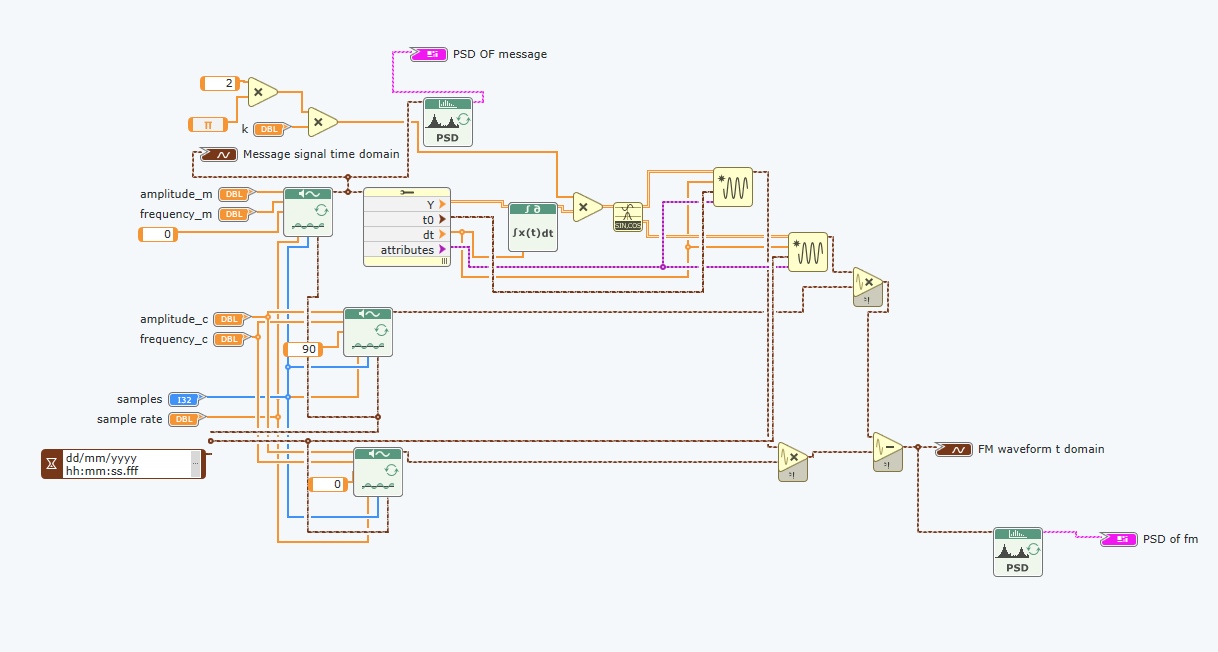
\includegraphics[width=1\textwidth]{FM_modulator.png}\end{center}

\vspace{0.5em}

\subsubsection{Block-by-Block Explanation}

\begin{enumerate}[leftmargin=2em]

\item \textbf{Sine Waveform (message signal generator)}
  \begin{itemize}[leftmargin=1.5em]
    \item \textbf{What it does:} Generates a single-tone sinusoidal waveform $m(t) = A_m \cos(2\pi f_m t)$.
    \item \textbf{Inputs wired:} Frequency $= 1$\,kHz, Amplitude $= 1$, Sample Rate $= 200$\,kHz, Samples $= 1000$.
    \item \textbf{Output:} A \texttt{Waveform} data type (array of samples + timing info: $dt$, $t_0$).
  \end{itemize}

\item \textbf{Waveform Properties}
  \begin{itemize}[leftmargin=1.5em]
    \item \textbf{What it does:} Extracts the array of Y-values, $dt$ (time step $= 1/f_s$), and $t_0$ from the waveform.
    \item \textbf{Why it matters:} We need the raw array $Y$ to do pointwise math, and we need $dt$ for the integrator.
    \item \textbf{Output:} Three terminals : \texttt{Y} (1D array of DBL), \texttt{dt} (DBL), \texttt{t0} (timestamp).
  \end{itemize}

\item \textbf{Integral x(t)}
  \begin{itemize}[leftmargin=1.5em]
    \item \textbf{What it does:} Numerically integrates the message array to compute $\int_0^t m(\tau)\,d\tau$.
    \item \textbf{Critical input:} Wire \texttt{dt} from Waveform Properties into the $dt$ terminal. Without this, the block assumes $dt = 1$ and the scaling is completely wrong.
    \item \textbf{After integration:} Multiply the output array by $2\pi k_f$ to get $\theta_m(t)$.
    \item \textbf{Output:} 1D array (same length as input).
  \end{itemize}

\item \textbf{Sine and Cosine}
  \begin{itemize}[leftmargin=1.5em]
    \item \textbf{What it does:} Takes the $\theta_m(t)$ array and computes $\cos(\theta_m(t))$ and $\sin(\theta_m(t))$ \emph{element-wise}.
    \item \textbf{Input:} The $2\pi k_f \int m(\tau)\,d\tau$ array.
    \item \textbf{Output:} Two 1D arrays : cosine values and sine values.
  \end{itemize}

\item \textbf{Carrier generation (two branches)}
  \begin{itemize}[leftmargin=1.5em]
    \item Generate time array $t = [0, dt, 2dt, \ldots]$ using the sample count and $dt$.
    \item Compute $\cos(2\pi f_c t)$ and $\sin(2\pi f_c t)$ for each sample.
    \item Multiply by $A_c$.
  \end{itemize}

\item \textbf{Multiply + Subtract}
  \begin{itemize}[leftmargin=1.5em]
    \item Compute: $A_c \cos(2\pi f_c t) \cdot \cos(\theta_m(t))$ (first term)
    \item Compute: $A_c \sin(2\pi f_c t) \cdot \sin(\theta_m(t))$ (second term)
    \item \textbf{Subtract} the second from the first to get $s(t)$.
  \end{itemize}

\item \textbf{Build Waveform}
  \begin{itemize}[leftmargin=1.5em]
    \item \textbf{What it does:} Re-packages the computed $s(t)$ array back into a \texttt{Waveform} data type by wiring $Y = s(t)$, $dt$, and $t_0$.
    \item \textbf{Why:} LabVIEW's graph indicators and PSD blocks expect waveform data types, not raw arrays.
  \end{itemize}

\item \textbf{PSD block (FFT Power Spectrum)}
  \begin{itemize}[leftmargin=1.5em]
    \item \textbf{What it does:} Computes the power spectral density of $s(t)$ using FFT.
    \item \textbf{Output:} Displayed on a graph indicator. This is what we compare across $k_f$ values.
  \end{itemize}

\item \textbf{Sub-VI creation}
  \begin{itemize}[leftmargin=1.5em]
    \item \textbf{Inputs to expose:} $f_m$, $A_m$, $f_c$, $A_c$, $k_f$, sample rate, samples.
    \item \textbf{Outputs to expose:} FM signal (time domain waveform), FM signal PSD.
  \end{itemize}

\end{enumerate}

\vspace{1.5em}

\subsection{Task 2: Observations for Different $k_f$ Values}

Parameters held constant: $f_m = 1$\,kHz, $f_c = 10$\,kHz, $f_s = 200$\,kHz, $N = 1000$, $A_m = 1$, $A_c = 1$.

\vspace{0.5em}

\subsubsection{$k_f = 500$ \; ($\mu = 0.5$, narrowband FM)}

\begin{center}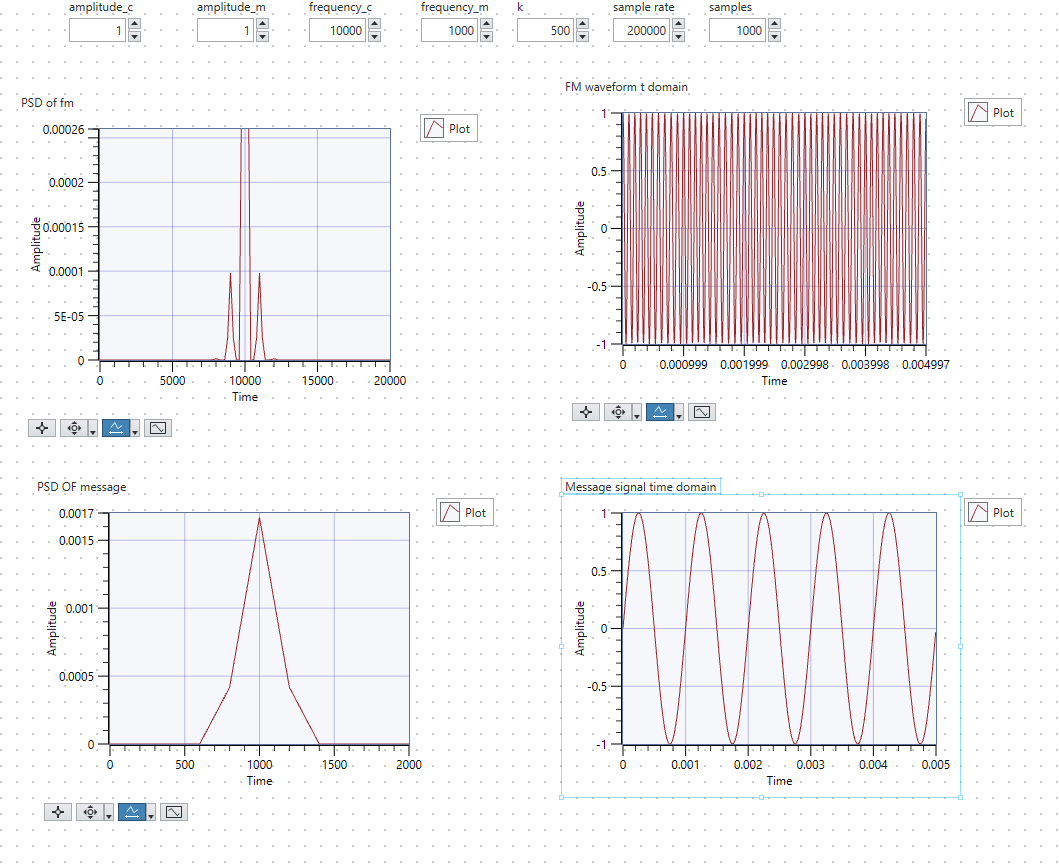
\includegraphics[width=0.5\textwidth]{kf_500.png}\end{center}

\textbf{Observations:}
\begin{itemize}[leftmargin=1.5em]
  \item \textbf{Time domain:} The waveform looks almost like a pure cosine at $f_c = 10$\,kHz. The frequency variation is subtle, we can barely see the compression/stretching of cycles.
  \item \textbf{PSD:} Dominated by a single peak at $f_c = 10$\,kHz with two small sidebands at $9$\,kHz and $11$\,kHz. Very similar to a DSB-AM spectrum.
\item \textbf{Why:} With $\mu = 0.5 < 1$, the phase deviation is small. From the formula derived earlier for the FM signal, we can see that for small values of $\mu$, the impact of $\sin$ is small, and thus the instantaneous frequency of the signal looks more constant at low values of $\mu$.

  \[
  s(t) = A_c \cos\!\Big(2\pi f_c t + \mu\sin(2\pi f_m t)\Big)
\]
  \item \textbf{Bandwidth:} Carson's rule gives $B_\text{FM} \approx 3$\,kHz, consistent with the result obtained.
\end{itemize}

\vspace{1em}

\subsubsection{$k_f = 2000$ \; ($\mu = 2$, wideband FM)}

\begin{center}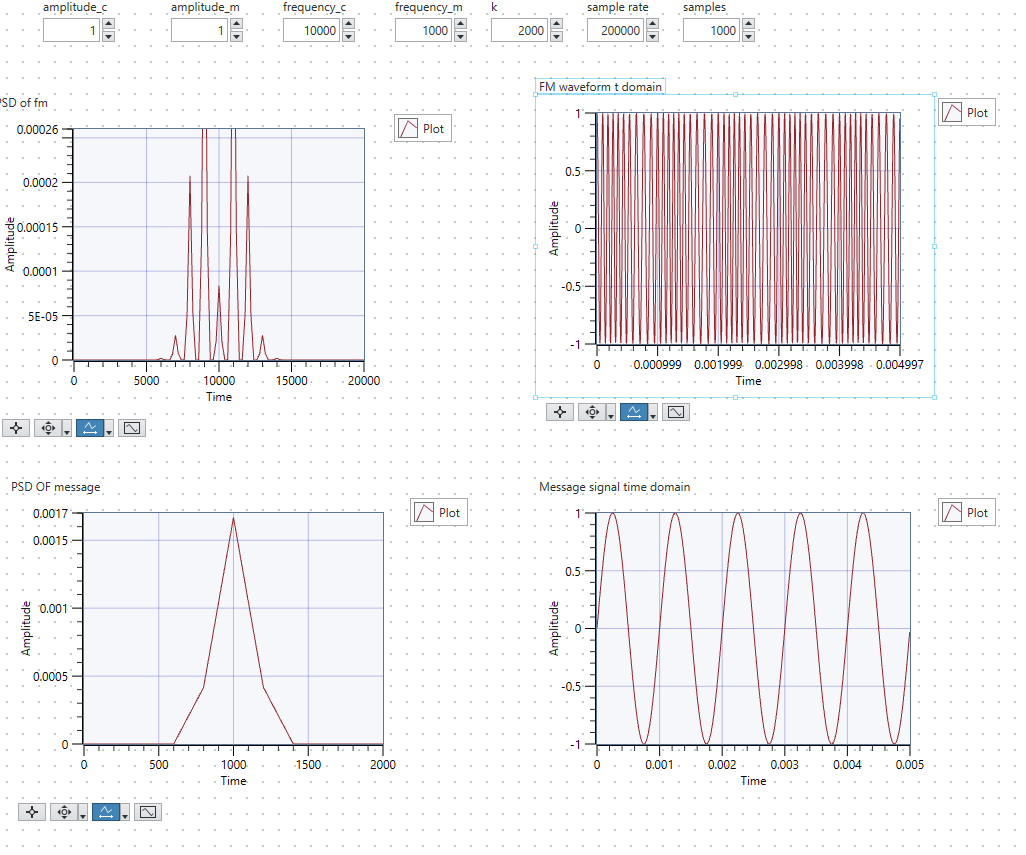
\includegraphics[width=0.5\textwidth]{kf_2000.png}\end{center}

\textbf{Observations:}
\begin{itemize}[leftmargin=1.5em]
  \item \textbf{Time domain:} Frequency variation is now visible. Where $m(t) > 0$, cycles are compressed (higher instantaneous frequency); where $m(t) < 0$, cycles are stretched (lower frequency). The envelope remains constant at $A_c = 1$.
  \item \textbf{PSD:} Multiple sidebands appear at $f_c \pm n \cdot 1$\,kHz for $n = 1, 2, 3$. The carrier peak at $10$\,kHz is reduced compared to $k_f = 500$, energy has redistributed into the sidebands.

  \item \textbf{Bandwidth:} Carson gives $B_\text{FM} \approx 6$\,kHz (sidebands from 7 to 13\,kHz visible).
\end{itemize}

\vspace{1em}

\subsubsection{$k_f = 5000$ \; ($\mu = 5$, wideband FM)}

\begin{center}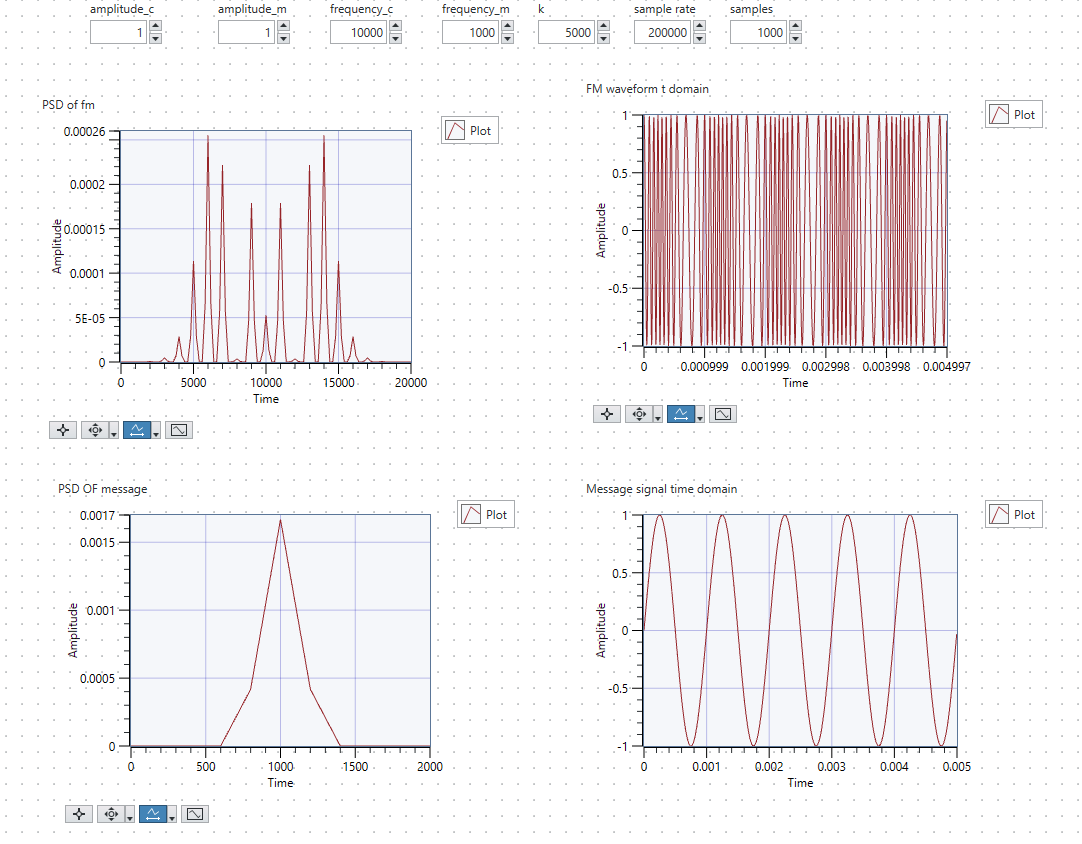
\includegraphics[width=0.5\textwidth]{kf_5000.png}\end{center}

\textbf{Observations:}
\begin{itemize}[leftmargin=1.5em]
  \item \textbf{Time domain:} Very pronounced frequency variation. The waveform is tightly compressed near message peaks and clearly stretched near troughs. Still constant envelope.
  \item \textbf{PSD:} Many sidebands (approximately $\mu + 1 = 6$ significant ones on each side). The spectrum spans roughly from 4\,kHz to 16\,kHz. The carrier component at 10\,kHz may be weaker than some sidebands (since $J_0(5) \approx -0.18$, i.e.\ the carrier amplitude is small).
  \item \textbf{Why:} Large $\mu$ means the instantaneous frequency deviates far from $f_c$, creating many harmonic components in the spectrum.
  \item \textbf{Bandwidth:} Carson gives $B_\text{FM} \approx 12$\,kHz, matching the observed spread.
\end{itemize}

\vspace{1.5em}

\begin{SummaryBox}[Exercise 1 Summary]
\begin{itemize}[leftmargin=1.5em]
  \item FM encodes information in \textbf{frequency}, not amplitude $\Rightarrow$ constant envelope.
  \item The LabVIEW implementation uses the trig expansion $s(t) = A_c\cos(2\pi f_c t)\cos(\theta_m) - A_c\sin(2\pi f_c t)\sin(\theta_m)$, where $\theta_m = 2\pi k_f \int m(\tau)\,d\tau$.
  \item Increasing $k_f$ increases $\Delta_f$ and $\mu$, which widens the spectrum and creates more sidebands.
  \item For $\mu < 1$ (narrowband), FM spectrum $\approx$ AM. For $\mu \gg 1$ (wideband), bandwidth grows as $2(\Delta_f + B)$.
  \item The sub-VI takes in signal parameters and $k_f$, outputs the FM waveform and its PSD.
\end{itemize}
\end{SummaryBox}

\newpage

\subsection{1.8 \; EXTRA: Bessel Function Interpretation of FM Spectra}

The exact spectrum of a single-tone FM signal can be derived by expanding $s(t) = A_c \cos(2\pi f_c t + \mu\sin(2\pi f_m t))$.

\textbf{Step 1:} Write the cosine as the real part of a complex exponential:
\[
  s(t) = \text{Re}\Big\{A_c\, e^{\,j(2\pi f_c t \,+\, \mu\sin(2\pi f_m t))}\Big\}
  = \text{Re}\Big\{A_c\, e^{\,j2\pi f_c t} \;\cdot\; e^{\,j\mu\sin(2\pi f_m t)}\Big\}
\]

\textbf{Step 2:} Apply the \textbf{Jacobi--Anger identity} to the second exponential, with $\phi = 2\pi f_m t$:
\[
  e^{\,j\mu\sin(\phi)} = \sum_{n=-\infty}^{\infty} J_n(\mu)\,e^{\,jn\phi}
\]
where $J_n(\mu)$ is the \textbf{Bessel function of the first kind}, order $n$. Substituting:
\[
  s(t) = \text{Re}\bigg\{A_c\, e^{\,j2\pi f_c t} \;\cdot\; \sum_{n=-\infty}^{\infty} J_n(\mu)\,e^{\,jn\,2\pi f_m t}\bigg\}
\]

\textbf{Step 3:} Combine the exponentials:
\[
  s(t) = \text{Re}\bigg\{A_c \sum_{n=-\infty}^{\infty} J_n(\mu)\,e^{\,j2\pi(f_c + n f_m)\,t}\bigg\}
\]

\textbf{Step 4:} Take the real part ($\text{Re}\{e^{j\theta}\} = \cos\theta$):
\[
\boxed{
  s(t) = A_c \sum_{n=-\infty}^{\infty} J_n(\mu)\,\cos\!\big(2\pi(f_c + n f_m)\,t\big)
}
\]

This tells us the FM spectrum consists of \textbf{discrete spectral lines} at frequencies $f_c + nf_m$ for $n = 0, \pm 1, \pm 2, \ldots$, each with amplitude $A_c\,J_n(\mu)$.

\vspace{0.5em}

\begin{center}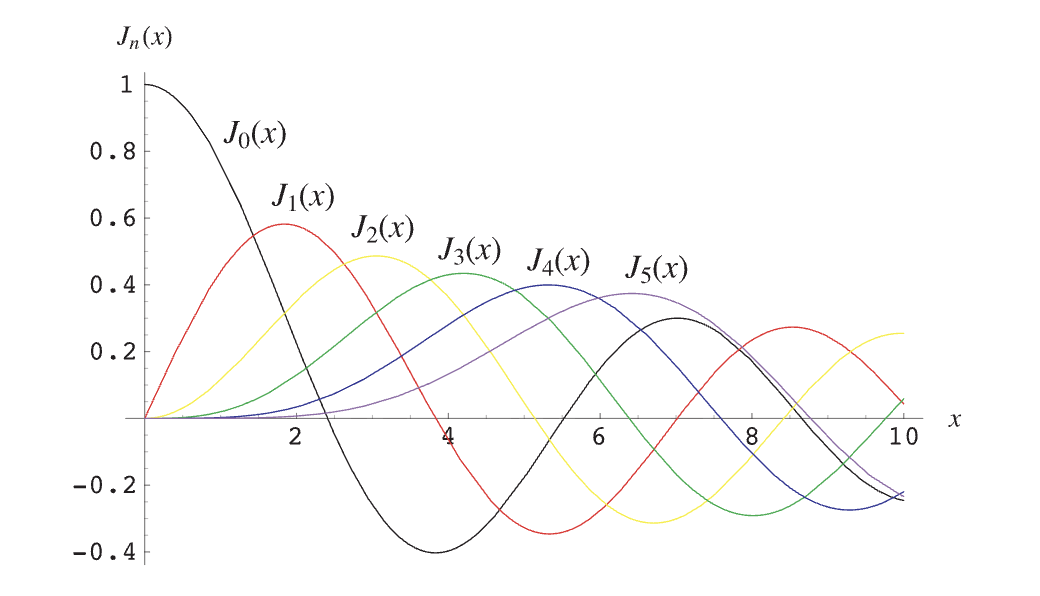
\includegraphics[width=0.8\textwidth]{besselfunctionsfirstkind.png}\end{center}

\vspace{0.5em}

\subsubsection{Key Properties of $J_n(\mu)$}

\begin{itemize}[leftmargin=1.5em]
\item \textbf{$n = 0$ (carrier frequency component):} The spectral amplitude at exactly $f_c$ is $A_c\,J_0(\mu)$. Although the time-domain envelope of the FM signal is always constant at $A_c$, the \textbf{power at the carrier frequency} varies with $\mu$, energy redistributes from the carrier into the sidebands as $\mu$ increases.

  \item \textbf{Carrier nulls:} $J_0(\mu) = 0$ at specific values of $\mu$. The first few zeros are:
  \[
    \mu \approx 2.405, \quad 5.520, \quad 8.654, \quad 11.792, \quad \ldots
  \]
  At these values, the carrier component \textbf{completely vanishes} from the spectrum, all the signal power sits in the sidebands.

  \item \textbf{Symmetry:} $J_{-n}(\mu) = (-1)^n J_n(\mu)$. This means sidebands at $f_c + nf_m$ and $f_c - nf_m$ have equal power (since power $\propto J_n^2$), but may differ in sign (phase).

  \item \textbf{Power conservation:} The total power is always $A_c^2/2$ regardless of $\mu$:
  \[
    \sum_{n=-\infty}^{\infty} J_n^2(\mu) = 1
  \]
  As $\mu$ increases, power does not increase, it \emph{redistributes} from the carrier into the sidebands.

  \item \textbf{Significant sidebands:} $J_n(\mu)$ becomes negligibly small for $|n| > \mu + 1$ (approximately). This is the mathematical basis of Carson's rule: $B_\text{FM} \approx 2(\mu + 1)f_m$.
\end{itemize}

\begin{center}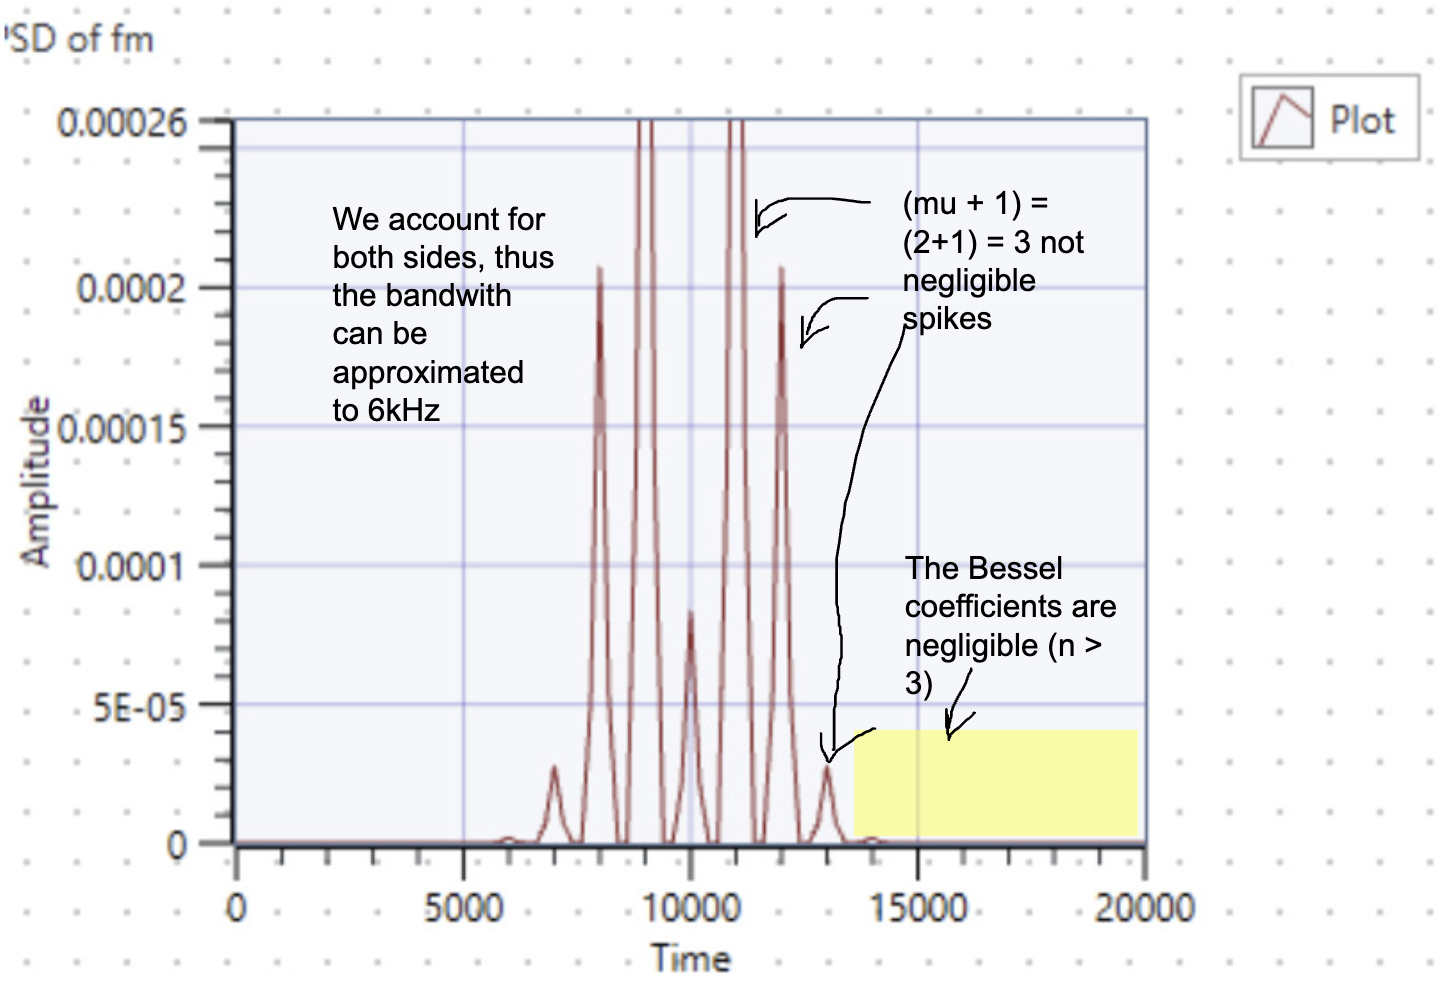
\includegraphics[width=0.8\textwidth]{analysis_mu2.png}\end{center}

\vspace{0.5em}

\subsubsection{Bessel Function Values for Our Lab Parameters}

\begin{center}
\renewcommand{\arraystretch}{1.2}
\begin{tabular}{c|ccccccc}
\toprule
$n$ & 0 & 1 & 2 & 3 & 4 & 5 & 6 \\
\midrule
$J_n(0.5)$ & 0.938 & 0.242 & 0.031 & 0.003 & --- & --- & --- \\
$J_n(2)$   & 0.224 & 0.577 & 0.353 & 0.129 & 0.034 & 0.007 & --- \\
$J_n(5)$   & $-0.178$ & $-0.328$ & 0.047 & 0.365 & 0.391 & 0.261 & 0.131 \\
\bottomrule
\end{tabular}
\end{center}

\textbf{Reading this table:}
\begin{itemize}[leftmargin=1.5em]
  \item $\mu = 0.5$: $J_0 = 0.938$ (strong carrier), $J_1 = 0.242$ (small sidebands), $J_2 \approx 0$ which confirms the narrowband approximation (Section~1.6): essentially just carrier + one pair of sidebands.
  \item $\mu = 2$: $J_0 = 0.224$ (carrier weakened), $J_1 = 0.577$ (first sideband is the strongest component). Energy has shifted away from the carrier.
  \item $\mu = 5$: $J_0 = -0.178$ (carrier is weak and phase-inverted), power is spread across many sidebands. $J_4 = 0.391$ is the strongest component which the dominant spectral line is not the carrier but the 4th sideband.
\end{itemize}

\newpage

\subsubsection{Extension Experiment 1: Carrier Null Observation}

\begin{GoalBox}[Extension: Carrier Null at $\mu = 2.405$]
\textbf{Prediction:} At $\mu = 2.405$, Bessel theory predicts $J_0(2.405) = 0$, so the carrier component at $f_c$ should vanish entirely from the PSD.

\textbf{Setup:} In the FM modulator sub-VI, we set $A_m = 1$, $f_m = 1$\,kHz, and choose $k_f$ such that:
\[
  \mu = \frac{k_f A_m}{f_m} = 2.405 \quad \Longrightarrow \quad k_f = 2405 \;\text{Hz}
\]

The peak at exactly $f_c$ should be \textbf{absent or near-zero}, while sidebands at $10 \pm 1$\,kHz, $10 \pm 2$\,kHz, etc.\ remain.

\textbf{Why this matters:} This is direct experimental confirmation that the carrier amplitude follows $J_0(\mu)$. It cannot be explained by Carson's rule alone, we need Bessel functions.
\end{GoalBox}

\begin{figure}[h]
\centering
\begin{subfigure}{0.7\textwidth}
    \centering
    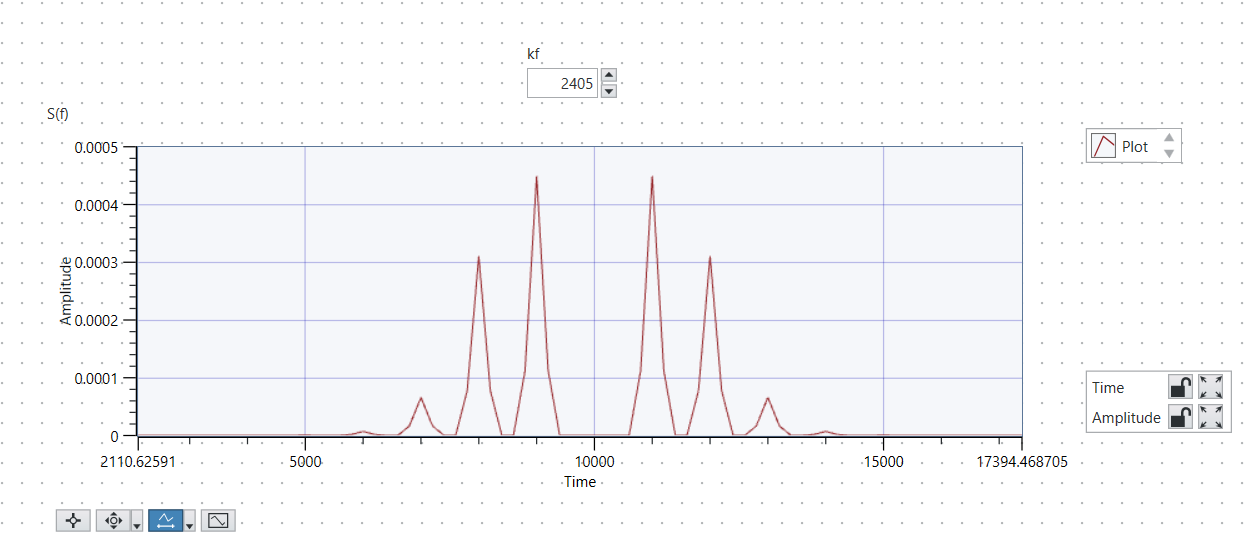
\includegraphics[width=\linewidth]{kf2405.png}
    \caption{$k_f = 2405$}
\end{subfigure}
\hfill
\begin{subfigure}{0.7\textwidth}
    \centering
    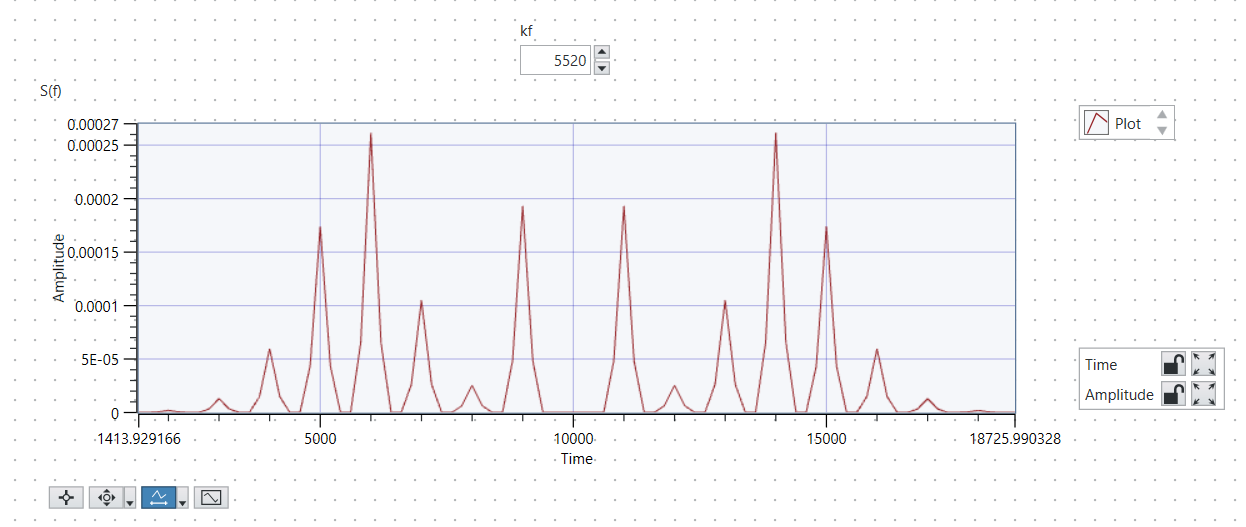
\includegraphics[width=\linewidth]{kf5520.png}
    \caption{$k_f = 5520$}
\end{subfigure}
\hfill
\begin{subfigure}{0.7\textwidth}
    \centering
    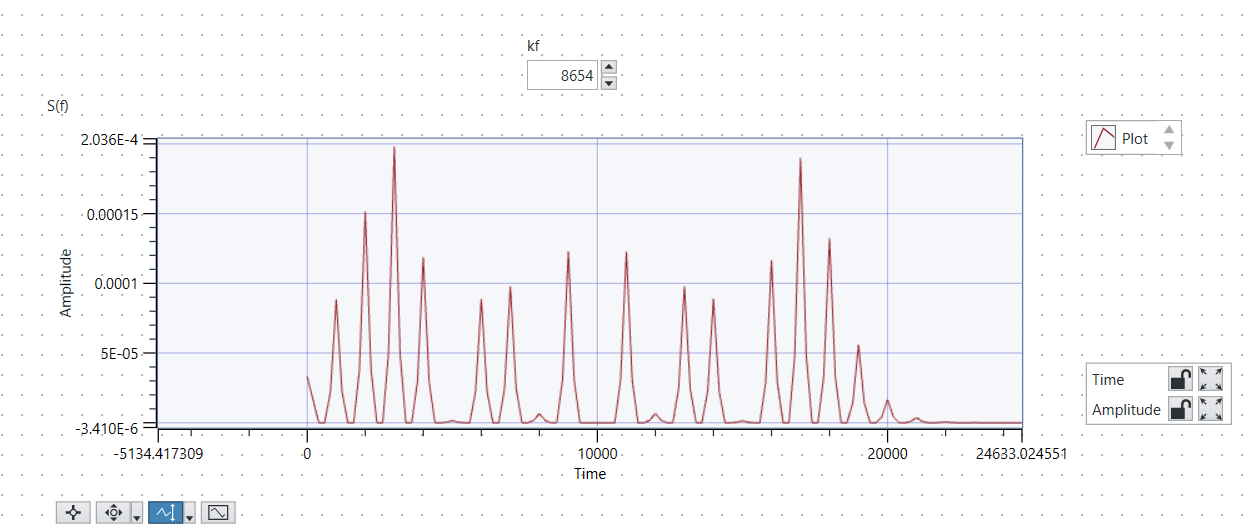
\includegraphics[width=\linewidth]{kf8654.png}
    \caption{$k_f = 8654$}
\end{subfigure}
\caption{Three images side by side}
\end{figure}

\vspace{1em}

\vspace{5em}

\begin{KeyBox}[Real-world Application of this Extension Experiment]

\textbf{1. Regulatory compliance.} When you transmit an FM signal, regulators (Ofcom in the UK, FCC in the US) define strict spectral masks, maximum allowed power at each frequency offset from your carrier. To prove your transmitter does not leak into adjacent channels, you need the exact power in each individual sideband. Bessel coefficients provide us with that: power in the $n$th sideband is proportional to $J_n^2(\mu)$. Carson's rule just says ``most power is within this range'',  that is not precise enough for a regulator.

\vspace{0.5em}

\textbf{2. Measuring $\mu$ experimentally (carrier null method).} You cannot read $\mu$ from the time-domain waveform because the envelope is always flat. But if you look at the spectrum and slowly increase $k_f$, at $\mu = 2.405$ the carrier peak vanishes because $J_0(2.405) = 0$. That gives you a precise known value of $\mu$. This is a real calibration technique used for FM transmitters,  you tune until the carrier disappears, and you know exactly what your modulation index is.

\vspace{0.5em}

\textbf{3. Receiver filter design.} The bandpass filter in the receiver must be wide enough to pass the significant sidebands, but narrow enough to reject noise and adjacent channels. Bessel coefficients tell you exactly which sidebands carry meaningful power and which are negligible, so you can choose the filter bandwidth precisely rather than relying on an approximation.

\vspace{0.5em}

\textit{Carson's rule $B_T \approx 2(\Delta_f + W)$ is a useful quick estimate, but it is not sufficient for real-world applications such as these, precise spectral engineering requires the full Bessel function analysis.}
\end{KeyBox}

\newpage

\section{Exercise 2: FM Demodulator: Conceptual Analysis}

\begin{GoalBox}[Goal of Exercise 2 (What we build)]
Build an FM demodulator sub-VI using \textbf{frequency discrimination}: differentiate the FM signal to turn frequency variations into amplitude variations (AM+FM), then envelope-detect to recover $m(t)$. This is the reverse of Exercise~1.
\end{GoalBox}

\vspace{1em}

\subsection{2.1 \; Frequency Discrimination: Full Derivation}

Start with the FM signal from Exercise~1:
\[
  s(t) = A_c \cos\!\big(2\pi f_c t + \phi(t)\big), \qquad \phi(t) = 2\pi k_f \int_0^t m(\tau)\,d\tau
\]

\subsubsection{Step 1: Differentiate the FM signal}

\begin{align}
  r(t) = \dot{s}(t)
  &= -A_c\Big[2\pi f_c + \dot{\phi}(t)\Big]\,\sin\!\big(2\pi f_c t + \phi(t)\big)
\end{align}

Since $\dot{\phi}(t) = 2\pi k_f m(t)$, this becomes:
\[
  r(t) = -A_c\Big[2\pi f_c + 2\pi k_f m(t)\Big]\,\sin\!\big(2\pi f_c t + \phi(t)\big)
\]

\begin{IntuitionBox}[Intuition to the algorithm :]
The differentiated signal is simultaneously \textbf{AM and FM} modulated:
\begin{itemize}[leftmargin=1.5em]
  \item The \textbf{amplitude envelope} is $A_c[2\pi f_c + 2\pi k_f m(t)]$ : it now carries $m(t)$.
  \item The carrier term $\sin(2\pi f_c t + \phi(t))$ still has FM modulation, but we don't care about it, the envelope detector will strip it away.
\end{itemize}
This is why the technique is called \textbf{frequency discrimination}: the differentiator converts frequency changes into amplitude changes.
\end{IntuitionBox}

\vspace{0.5em}

\subsubsection{Step 2: Envelope detection}

The envelope detector extracts the amplitude envelope:
\[
  q(t) = A_c\Big[2\pi f_c + 2\pi k_f m(t)\Big]
\]

This contains a large \textbf{DC component} ($A_c \cdot 2\pi f_c$) plus the desired signal ($A_c \cdot 2\pi k_f m(t)$).

\subsubsection{Step 3: Remove DC and scale}

After removing the DC offset (via AC coupling or subtracting the mean):
\[
  u(t) = A_c \cdot 2\pi k_f \cdot m(t)
\]

Divide by the known constant $2\pi k_f A_c$:
\[
\boxed{y(t) = m(t)}
\]

\begin{KeyBox}[Key Result: FM Demodulation Chain]
\[
  s(t) \;\xrightarrow{\;\text{differentiate}\;}\; r(t) \;\xrightarrow{\;\text{envelope detect}\;}\; q(t) \;\xrightarrow{\;\text{remove DC, scale}\;}\; m(t)
\]
\end{KeyBox}

\vspace{0.5em}

\newpage

\section{Exercise 2: FM Demodulator --- Task Answers}

\subsection{Task 1: LabVIEW Block Diagram}

\begin{center}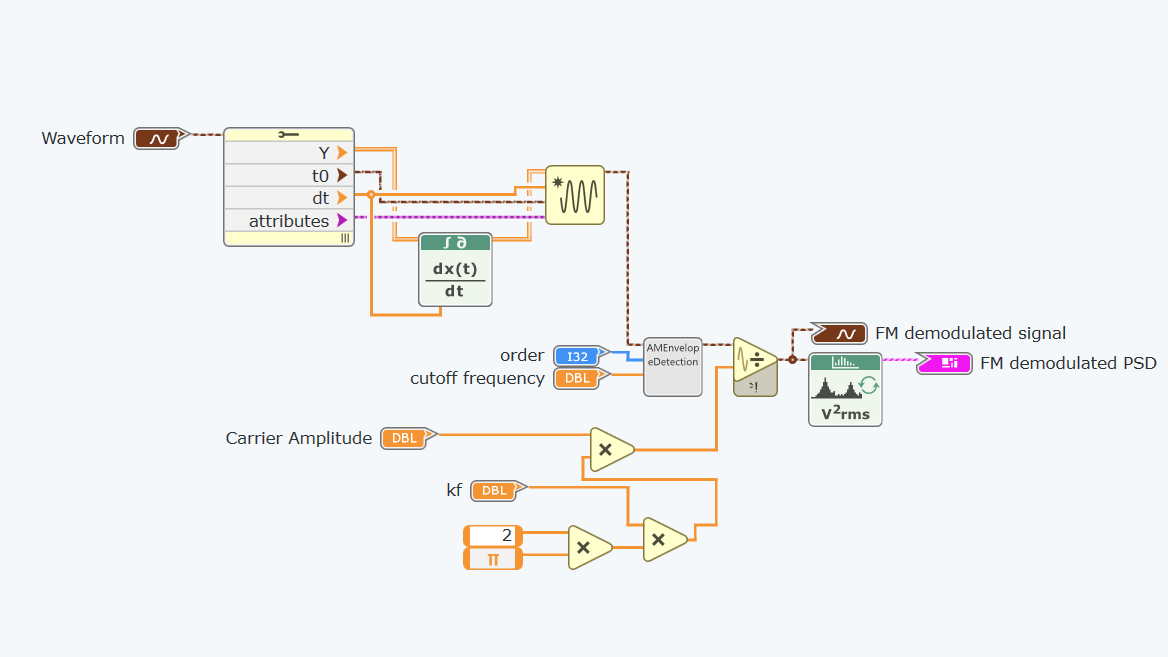
\includegraphics[width=0.5\textwidth]{FM_demodulator.png}\end{center}

\vspace{0.5em}

\subsubsection{Block-by-Block Explanation}

The demodulator receives the FM waveform from the modulator sub-VI and outputs the recovered message.

\begin{enumerate}[leftmargin=2em]

\item \textbf{Waveform Properties (input side)}
  \begin{itemize}[leftmargin=1.5em]
    \item Unpacks the incoming FM waveform into \texttt{Y} (sample array), \texttt{dt}, and \texttt{t0}.
    \item We need \texttt{dt} for the derivative block.
  \end{itemize}

\item \textbf{Derivative x(t)}
  \begin{itemize}[leftmargin=1.5em]
    \item \textbf{What it does:} Numerically differentiates the FM signal array, computing $\dot{s}(t)$.
    \item \textbf{Critical input:} Wire \texttt{dt} into its $dt$ terminal, just like the integrator in Exercise~1. Without this, the derivative scaling is wrong.
    \item \textbf{Output:} 1D array representing $r(t) = A_c[2\pi f_c + 2\pi k_f m(t)]\sin(2\pi f_c t + \phi(t))$.
    \item This is the AM+FM signal.
  \end{itemize}

\item \textbf{Butterworth Low-Pass Filter}
  \begin{itemize}[leftmargin=1.5em]
    \item \textbf{What it does:} Smooths the signal after rectification, removing the high-frequency carrier components and keeping only the baseband envelope.
    \item \textbf{Inputs:} Order $= 5$, cutoff frequency $= 1400$\,Hz (just above $f_m = 1$\,kHz to pass the message but reject carrier at $f_c = 10$\,kHz).
    \item \textbf{Why Butterworth?} Maximally flat passband (no ripple), so the recovered message is not distorted.
  \end{itemize}

\item \textbf{AM Envelope Detection (from Lab 2)}
  \begin{itemize}[leftmargin=1.5em]
    \item \textbf{What it does:} Extracts the amplitude envelope of the AM+FM signal. This is the same sub-VI built in Lab~2 Exercise~1b .
    \item \textbf{Output:} The envelope $q(t) \propto [2\pi f_c + 2\pi k_f m(t)]$ plus a DC offset.
  \end{itemize}

\item \textbf{DC removal}
  \begin{itemize}[leftmargin=1.5em]
    \item Subtract the mean of the envelope signal to remove the $2\pi f_c A_c$ constant.
    \item After this step, only $A_c \cdot 2\pi k_f \cdot m(t)$ remains.
  \end{itemize}

\item \textbf{Amplitude scaling}
  \begin{itemize}[leftmargin=1.5em]
    \item Multiply by $\dfrac{1}{2\pi \cdot k_f \cdot A_c}$ to recover $m(t)$ with correct amplitude.
  \end{itemize}

\item \textbf{Build Waveform + PSD}
  \begin{itemize}[leftmargin=1.5em]
    \item Re-package the demodulated array into a waveform (wire Y, dt, t0).
    \item Compute PSD of the demodulated signal for the frequency-domain indicator.
  \end{itemize}

\item \textbf{Sub-VI creation}
  \begin{itemize}[leftmargin=1.5em]
    \item \textbf{Inputs:} FM signal (waveform), $k_f$, $A_c$, filter order, filter cutoff frequency.
    \item \textbf{Outputs:} Demodulated signal (time domain waveform), demodulated signal PSD.
  \end{itemize}

\end{enumerate}

\vspace{1em}

\begin{SummaryBox}[Exercise 2 Summary]
\begin{itemize}[leftmargin=1.5em]
  \item FM demodulation via \textbf{frequency discrimination} = differentiate + envelope detect + scale.
  \item Differentiation converts FM into AM+FM; envelope detection extracts the message from the amplitude.
  \item Scaling by $1/(2\pi k_f A_c)$ recovers the original message amplitude.
  \item The Butterworth LPF (order 5, $f_\text{cutoff} = 1400$\,Hz) cleans up the output.
\end{itemize}
\end{SummaryBox}

\newpage

\section{Exercise 3: FM Simulation: Conceptual Analysis}

\begin{GoalBox}[Goal of Exercise 3 (What we build)]
Combine the FM Modulator (Exercise~1) and FM Demodulator (Exercise~2) sub-VIs into a single top-level VI (\texttt{FMTopLevel.gvi}) to observe the complete FM modulation $\to$ demodulation chain in real-time.
\end{GoalBox}

\vspace{1em}

\subsection{3.1 \; What This Exercise Adds}

This is an \textbf{integration exercise}, no new theory, just wiring the two sub-VIs together and wrapping them in a while loop.

The signal flow is:

\[
  m(t) \;\xrightarrow{\;\text{FM Modulator sub-VI}\;}\; s(t) \;\xrightarrow{\;\text{FM Demodulator sub-VI}\;}\; \hat{m}(t)
\]

\begin{itemize}[leftmargin=1.5em]
  \item The modulator sub-VI outputs the FM waveform, the carrier waveform, the message waveform, their PSDs, and the modulation index $\mu$.
  \item The demodulator sub-VI receives the FM waveform and outputs the demodulated signal and its PSD.
\end{itemize}

\vspace{0.5em}

\subsection{3.2 \; Simulation Parameters}

\begin{center}
\begin{tabular}{lc}
\toprule
\textbf{Parameter} & \textbf{Value} \\
\midrule
Message frequency $f_m$ & 1\,kHz \\
Carrier frequency $f_c$ & 10\,kHz \\
Sample rate $f_s$ & 200\,kHz \\
Number of samples $N$ & 1000 \\
Butterworth filter order & 5 \\
Butterworth cutoff frequency & 1400\,Hz \\
\bottomrule
\end{tabular}
\end{center}

\vspace{0.5em}

\textbf{Why cutoff = 1400\,Hz?}

After the envelope detector, the output is not perfectly clean, there are residual high-frequency components at and around $f_c = 10$\,kHz leaking through (carrier remnants that the envelope detector did not fully remove). The Butterworth LPF's job is to suppress those while passing the 1\,kHz message. The cutoff just needs to be \textbf{above 1\,kHz} (to pass the message) and \textbf{low enough} that the filter's roll-off has attenuated the 10\,kHz components to negligible levels.

1400\,Hz is the sweet spot: comfortably above 1\,kHz, and with a 5th-order Butterworth ($100$\,dB/decade roll-off), the attenuation at 10\,kHz is already massive.

\newpage

\section{Exercise 3: FM Simulation: Task Answers}

\subsection{Task 1: Top-Level Block Diagram}

\begin{center}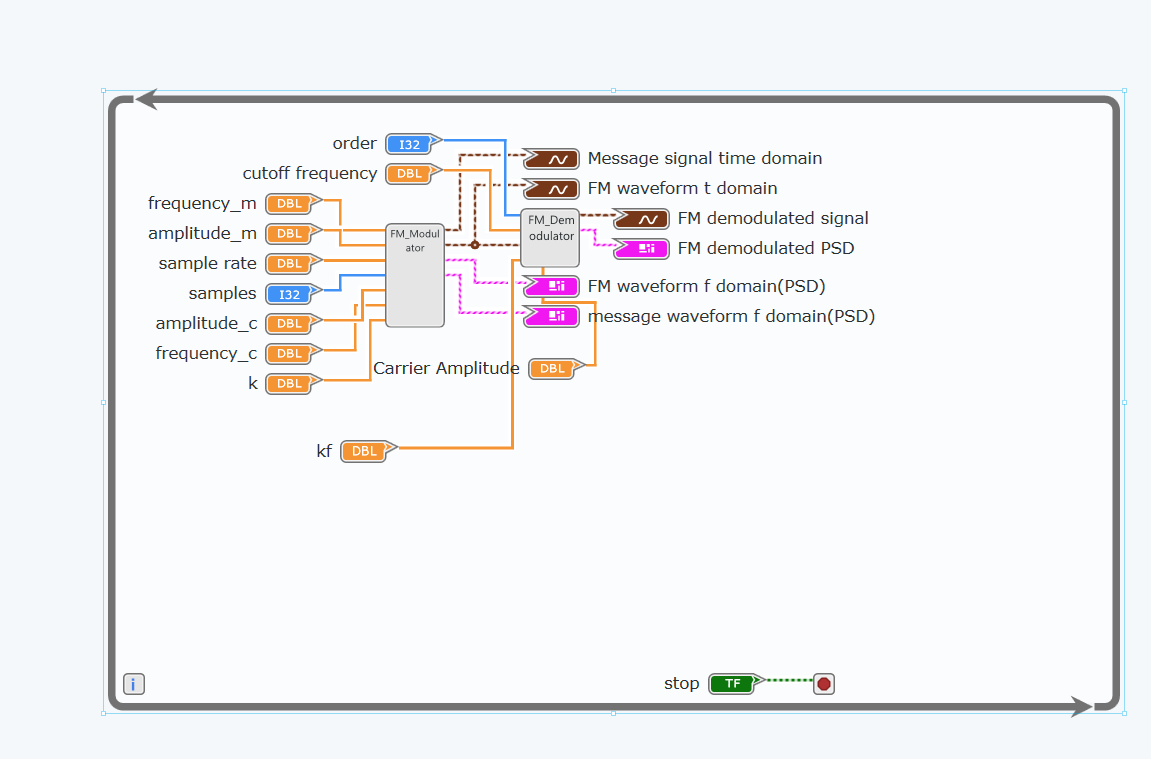
\includegraphics[width=0.5\textwidth]{FM_full.png}\end{center}

\subsubsection{Block-by-Block Explanation}

\begin{enumerate}[leftmargin=2em]

\item \textbf{Front panel controls (left side)}
  \begin{itemize}[leftmargin=1.5em]
    \item Numeric controls for: Sample Rate, Samples Number, Timestamp t0, Message Amplitude, Message Frequency, Carrier Amplitude, Carrier Frequency, Frequency Sensitivity ($k_f$), filter order, filter cutoff frequency.
    \item A \textbf{Stop} button (boolean) wired to the while loop's stop terminal.
  \end{itemize}

\item \textbf{FM Modulator sub-VI}
  \begin{itemize}[leftmargin=1.5em]
    \item Receives all signal parameters from the front panel controls.
    \item Outputs: FM waveform, carrier waveform, message waveform, their PSDs, and the computed modulation index $\mu = k_f A_m / f_m$.
  \end{itemize}

\item \textbf{FM Demodulator sub-VI}
  \begin{itemize}[leftmargin=1.5em]
    \item Receives the FM waveform from the modulator, plus $k_f$, $A_c$, filter order, and cutoff frequency.
    \item Outputs: demodulated signal waveform and its PSD.
  \end{itemize}

\item \textbf{Graph indicators (right side)}
  \begin{itemize}[leftmargin=1.5em]
    \item Message Signal (time) + its PSD
    \item Carrier Signal (time)
    \item FM Modulated Signal (time) + its PSD
    \item Demodulated Signal (time) + its PSD
  \end{itemize}

\item \textbf{While loop + Stop button}
  \begin{itemize}[leftmargin=1.5em]
    \item Everything sits inside a while loop. The stop button breaks the loop.
    \item Each iteration recomputes the full modulation--demodulation chain with the current front panel values.
  \end{itemize}

\end{enumerate}

\vspace{1em}

\subsection{Task 2: Front Panel and Observations}

\begin{center}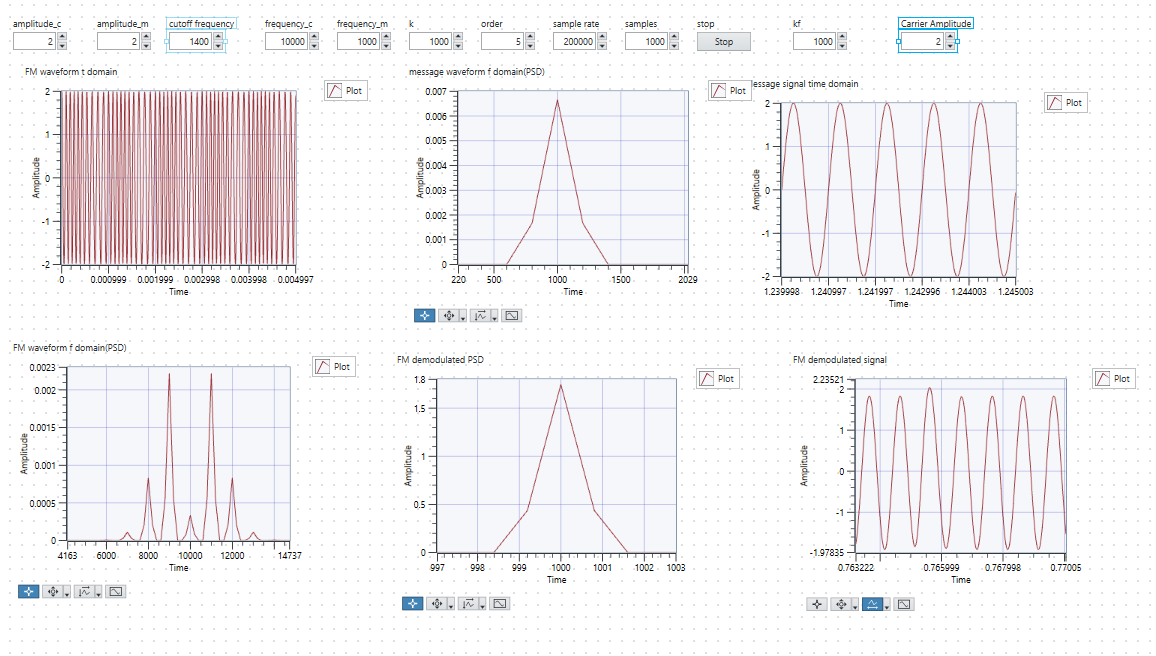
\includegraphics[width=0.8\textwidth]{FM_simulation_results.png}\end{center}

\textbf{Observations:}
\begin{itemize}[leftmargin=1.5em]
  \item \textbf{Message signal:} Clean sinusoid at 1\,kHz with amplitude $A_m$. PSD shows a single peak at 1\,kHz.
  \item \textbf{Carrier signal:} Pure sinusoid at 10\,kHz with amplitude $A_c$.
  \item \textbf{FM signal:} Constant-envelope waveform with visible frequency variation. PSD shows sidebands whose spread depends on $k_f$ (as explored in Exercise~1).
  \item \textbf{Demodulated signal:} Recovers the original 1\,kHz sinusoid. The initial transient from the Butterworth filter is visible at the start. After settling, amplitude matches $A_m$.
  \item \textbf{Demodulated PSD:} Single clean peak at 1\,kHz, confirming faithful recovery of the message.
  \item \textbf{Real-time tweaking:} Increasing $k_f$ on the front panel immediately widens the FM spectrum and (as long as the filter cutoff is set properly) the demodulated output remains correct.
\end{itemize}

\vspace{0.5em}

\begin{SummaryBox}[Exercise 3 Summary]
\begin{itemize}[leftmargin=1.5em]
  \item Exercise~3 is purely an \textbf{integration exercise}: wire the modulator and demodulator sub-VIs together.
  \item The end-to-end chain confirms: FM modulation preserves the message in the frequency, and frequency discrimination faithfully recovers it.
  \item The Butterworth filter parameters (order~5, cutoff 1400\,Hz) are critical, too low cuts the message, too high lets carrier leakage through.
\end{itemize}
\end{SummaryBox}

\newpage

\section{Exercise 4: FM Communications via USRP : Conceptual Analysis}

\begin{GoalBox}[Goal of Exercise 4 (What we build)]
Use the provided \texttt{FM-TxRx.gvi} to transmit and receive FM signals over the air using the USRP hardware. This is the first time \textbf{real noise} enters the system , unlike Exercises~1--3 which were pure simulation.
\end{GoalBox}

\vspace{1em}

\subsection{4.1 \; How FM-TxRx.gvi Differs from the Simulation}

The provided VI combines transmission and reception in a \textbf{single VI} with two while loops running simultaneously (LabVIEW executes parallel while loops concurrently). The signal flow is identical to our simulation:

\begin{itemize}[leftmargin=1.5em]
  \item \textbf{TX loop:} message $\to$ FM modulation (same math as Exercise~1) $\to$ \texttt{niUSRP Write Tx Data} (sends complex baseband samples to the USRP hardware, which upconverts to RF).
  \item \textbf{RX loop:} \texttt{niUSRP Fetch Rx Data} (receives RF, downconverts to complex baseband) $\to$ FM demodulation (same discriminator as Exercise~2) $\to$ display.
\end{itemize}

\begin{IntuitionBox}[Simulation vs.\ USRP: what changes?]
In the simulation (Exercise~3), the FM waveform goes directly from modulator to demodulator, there is no noise. With the USRP, the signal travels \emph{over the air}: the USRP transmitter upconverts to RF, the signal propagates through a wireless channel (with attenuation and additive noise), and the USRP receiver downconverts back. This introduces \textbf{real channel noise}, making gain settings critical.
\end{IntuitionBox}

\vspace{1em}

\subsection{4.2 \; FM Output SNR : Why FM Handles Noise Well}

Since this is the first exercise with real noise, here is the key result from the lectures.

At the output of an FM receiver (after the discriminator + LPF), the signal and noise powers are:
\[
  P_S = k_f^2 P, \qquad P_N = \frac{2N_0 W^3}{3A^2}
\]
where $P = \overline{m^2(t)}$ is the message power, $W$ is the message bandwidth, $A$ is the carrier amplitude, and $N_0$ is the noise spectral density.

\begin{KeyBox}[Key: FM Output SNR]
\[
  \text{SNR}_\text{FM} = \frac{P_S}{P_N} = \frac{3A^2 k_f^2 P}{2N_0 W^3}
  = 3\beta^2 \frac{P}{m_p^2}\;\text{SNR}_\text{baseband}
\]
where $\text{SNR}_\text{baseband} = \dfrac{A^2}{2N_0 W}$ and $\beta = \dfrac{k_f m_p}{W}$.

Key takeaways:
\begin{itemize}[leftmargin=1.5em]
  \item $\text{SNR}_\text{FM} \propto \beta^2$: \textbf{quadratic} improvement with modulation index, much better than AM.
  \item $P_N \propto 1/A^2$: increasing carrier power reduces noise (\textbf{noise-quieting effect}).
  \item This is valid for high SNR (above the FM threshold, $\rho \approx 10$).
\end{itemize}
\end{KeyBox}

\vspace{0.5em}

\textbf{Why does noise PSD grow as $f^2$?}

\begin{KeyBox}[EXTRA : Noise PSD After the Discriminator]

The discriminator output is:
\[
  v(t) = \frac{1}{2\pi}\frac{d\theta(t)}{dt} \approx k_f m(t) + n_d(t)
\]

where the additive noise term is:
\[
  n_d(t) = \frac{1}{2\pi A}\frac{d}{dt}\Big[r(t)\sin\!\big(\psi(t) - \phi(t)\big)\Big]
  \approx \frac{1}{2\pi A}\frac{d}{dt}\Big[r(t)\sin\!\big(\psi(t)\big)\Big]
  = \frac{1}{2\pi A}\frac{d}{dt}n_Q(t)
\]

The approximation holds at high SNR ($A \gg r(t)$), where $\phi(t)$ can be dropped. Since $r(t)\sin(\psi(t)) = n_Q(t)$ (the quadrature component of the narrowband noise), the discriminator noise reduces to a \textbf{scaled derivative of $n_Q(t)$}.

\textbf{PSD:} differentiation in time multiplies the spectrum by $(2\pi f)^2$, so:
\[
  S_{N_0}(f) = \left(\frac{1}{2\pi A}\right)^{\!2}(2\pi f)^2\,S_{N_Q}(f)
  = \frac{f^2}{A^2}\,N_0, \qquad |f| \leq W
\]

This is a \textbf{parabolic} noise PSD :  high-frequency noise is amplified far more than low-frequency noise.

\begin{center} 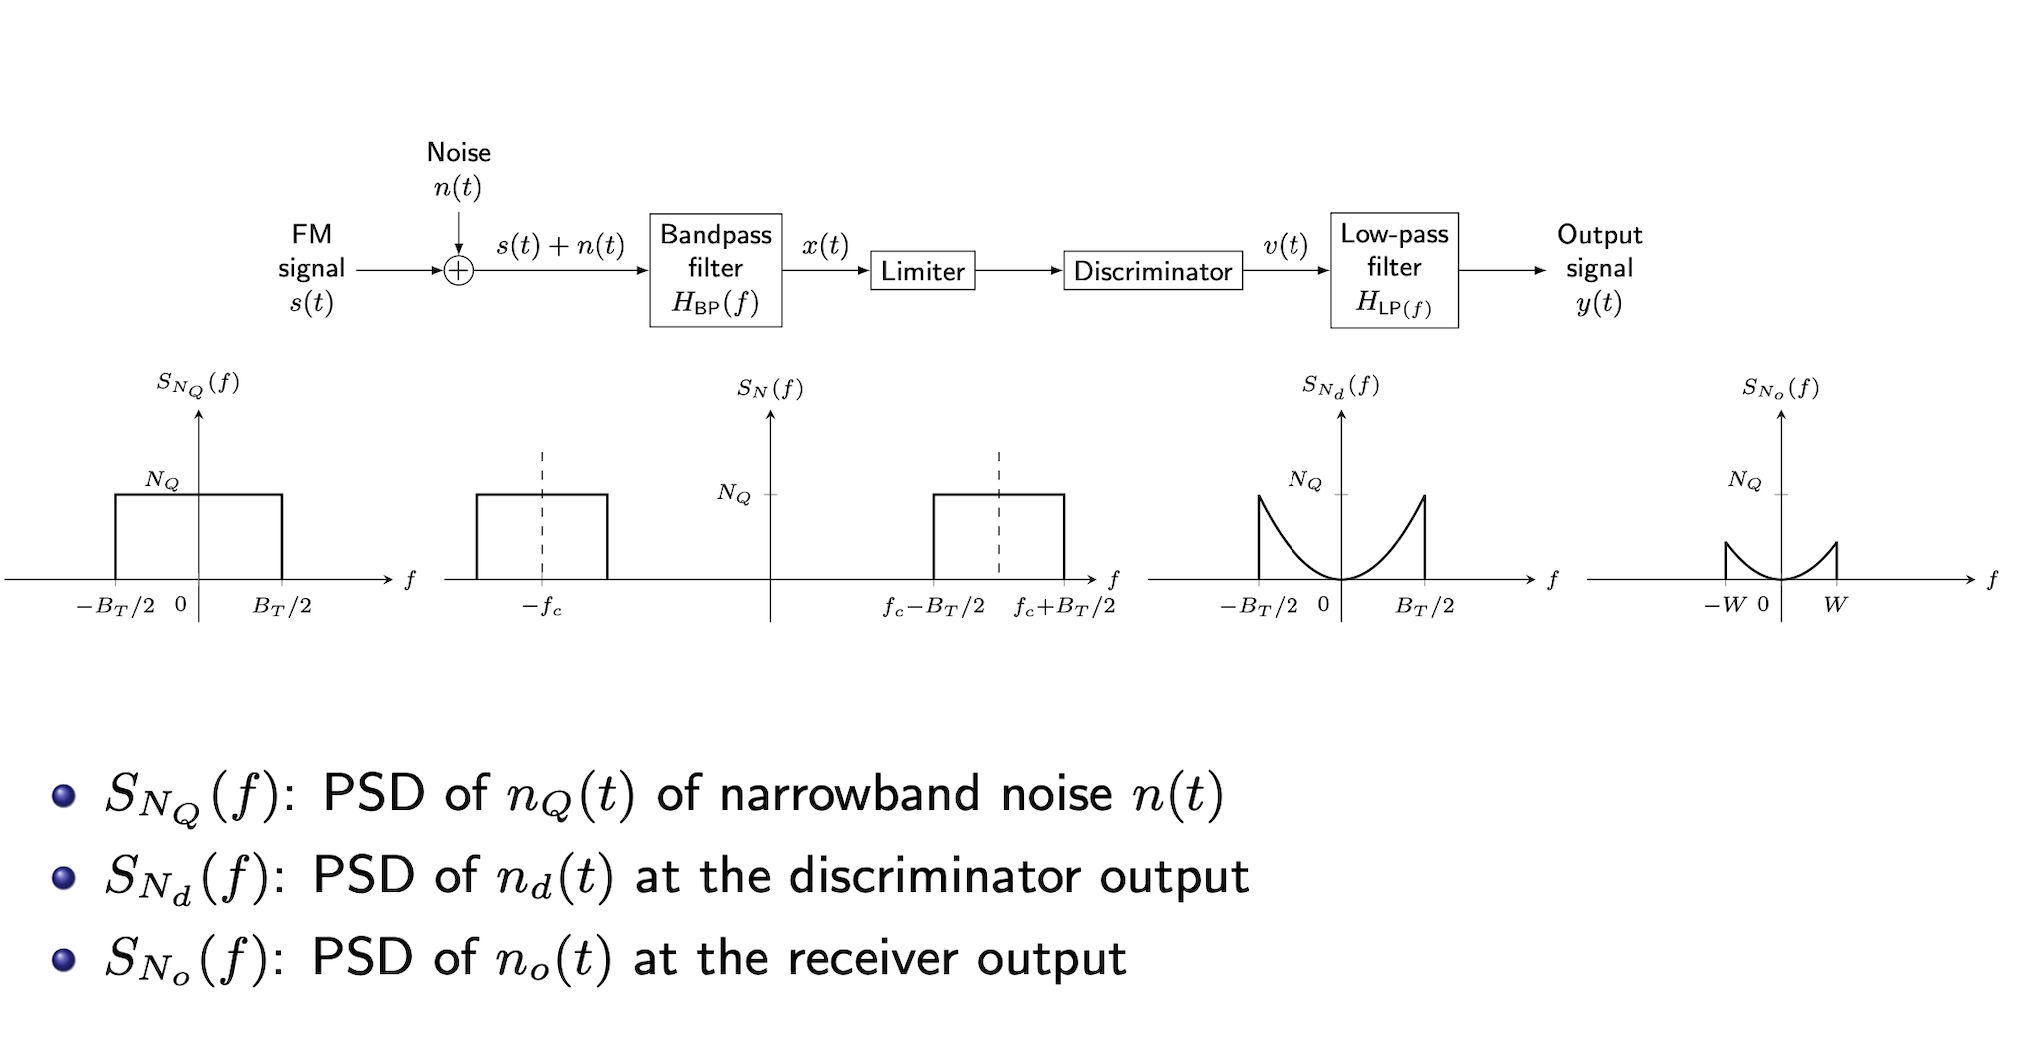
\includegraphics[width=0.7\textwidth]{lecture8_slide14_noise_psd.png} \end{center}
\end{KeyBox}

\vspace{3em}

\textbf{ Noise-quieting effect :} The noise power $P_N \propto 1/A^2$ means that as we increase the carrier amplitude (i.e.\ increase transmit gain on the USRP), the output noise \emph{decreases}. This is a unique property of FM not shared by AM. In the lab, we observe this directly: increasing the USRP gain cleans up the demodulated signal.

\newpage

\section{Exercise 4: FM Communications via USRP : Task Answers}

\subsection{Task 1: Block Diagram }

 \begin{center} 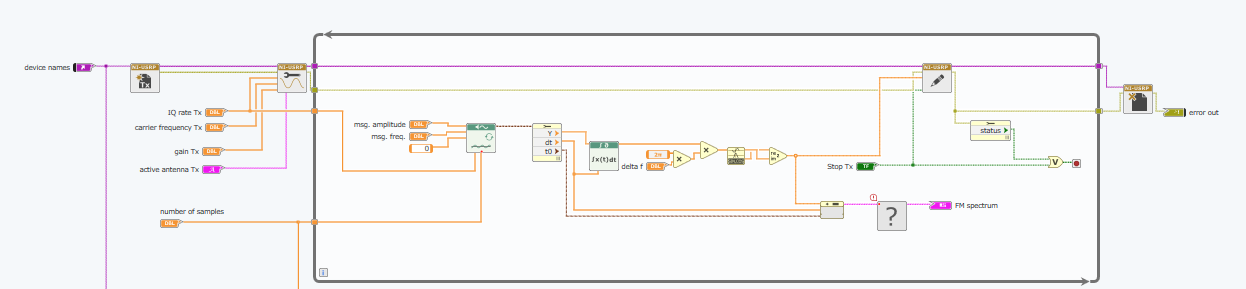
\includegraphics[width=0.7\textwidth]{FM_USRP_block1.png} \end{center}

  \begin{center} 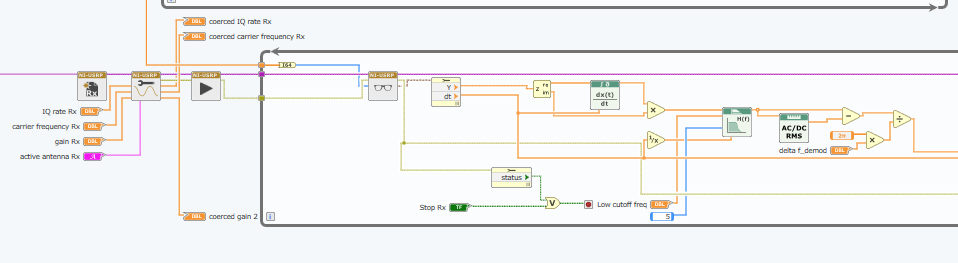
\includegraphics[width=0.7\textwidth]{FM_USRP_block2.png} \end{center}

   \begin{center} 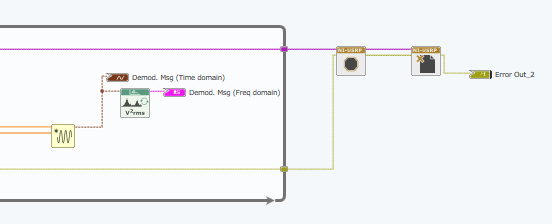
\includegraphics[width=0.7\textwidth]{FM_USRP_block3.png} \end{center}

\textbf{Comparison with simulation (Exercise 3):}
\begin{itemize}[leftmargin=1.5em]
  \item The \textbf{modulation and demodulation math is identical}, same trig expansion, same discriminator + envelope detection.
  \item The key difference is the \textbf{USRP hardware interface}: \texttt{niUSRP Write Tx Data} replaces the direct wire between modulator and demodulator. \texttt{niUSRP Fetch Rx Data} captures samples from the antenna.
  \item Both TX and RX sit in separate while loops that run \textbf{simultaneously} (LabVIEW's parallel execution).
  \item Additional controls: \textbf{carrier frequency} (set to a frequency agreed upon in the lab), \textbf{IQ rate} (sample rate for the USRP), \textbf{gain} (TX and RX).
\end{itemize}

\vspace{1em}

\newpage

\section{Exercise 4a: Carson's Rule : Conceptual Analysis}

\begin{GoalBox}[Goal of Exercise 4a]
Experimentally validate \textbf{Carson's rule} by measuring the FM bandwidth from the USRP power spectrum at three different frequency deviations ($\Delta_f = 1, 5, 30$\,kHz) and comparing to the theoretical prediction.
\end{GoalBox}

\vspace{1em}

\subsection{4a.1 \; Carson's Rule (Demonstrated in the extension for exercice 1) }

The exact bandwidth of an FM signal is theoretically infinite (infinitely many Bessel sidebands). In practice, most of the power ($\approx 98\%$) is contained within a finite bandwidth approximated by:

\[
\boxed{
  B_T \;=\; 2(\Delta_f + W) \;=\; 2W(\beta + 1)
}
\]

where $\Delta_f = k_f m_p$ is the frequency deviation and $W$ is the message bandwidth.

\textbf{Limiting cases:}
\begin{itemize}[leftmargin=1.5em]
  \item $\beta \ll 1$ (narrowband FM): $B_T \approx 2W$ , same as AM. The spectrum has just two sidebands.
  \item $\beta \gg 1$ (wideband FM): $B_T \approx 2\Delta_f$ , bandwidth is dominated by the frequency deviation, not the message bandwidth.
\end{itemize}

\vspace{0.5em}

\subsection{4a.2 \; Spectrum Appearance on the USRP}

The ``FM spectrum'' graph on the USRP front panel shows the \textbf{baseband-equivalent} spectrum: the carrier appears at 0\,Hz (not at $f_c$), with lower sideband on the negative-frequency side and upper sideband on the positive side. This is the standard baseband representation after downconversion.

For a single-tone message at $f_m = 1$\,kHz, the spectrum consists of discrete spectral lines at $n \times 1$\,kHz, $n = 0, \pm 1, \pm 2, \ldots$, with amplitudes given by Bessel functions $J_n(\beta)$.

\vspace{0.5em}

\subsection{4a.3 \; Predicted vs.\ Measured Bandwidth}

\begin{center}
\renewcommand{\arraystretch}{1.3}
\begin{tabular}{cccccc}
\toprule
$\Delta_f$ (kHz) & $W$ (kHz) & $\beta = \Delta_f / W$ & Regime & $B_T = 2(\Delta_f + W)$ & Measured $B_T$ \\
\midrule
1  & 1 & 1  & Narrowband & 4\,kHz  & $\sim$4\,kHz \\
5  & 1 & 5  & Wideband   & 12\,kHz & $\sim$14\,kHz \\
30 & 1 & 30 & Wideband   & 62\,kHz & $\sim$70\,kHz \\
\bottomrule
\end{tabular}
\end{center}

\begin{IntuitionBox}[Why is the measured bandwidth slightly larger than Carson's prediction?]
Carson's rule captures $\approx 98\%$ of the power. The remaining $\sim$2\% sits in outer sidebands that are visible on the spectrum analyser. Carson's rule is a \textbf{lower bound} approximation.
\end{IntuitionBox}

\vspace{0.5em}

\textbf{Low $\Delta_f$ distortion :} At low frequency deviation ($\Delta_f = 1$\,kHz) incurs distortion. This is because a small $\Delta_f$ means the frequency changes corresponding to the message amplitude are small. The reduced bandwidth may not capture all the modulated signal's nuances, and the discriminator output has a lower SNR (recall $\text{SNR}_\text{FM} \propto \beta^2$: low $\beta$ means low SNR).

\newpage

\section{Exercise 4a: Carson's Rule: Task Answers}

\subsection{Task 1: Power Spectrum Plots}

 \begin{center} 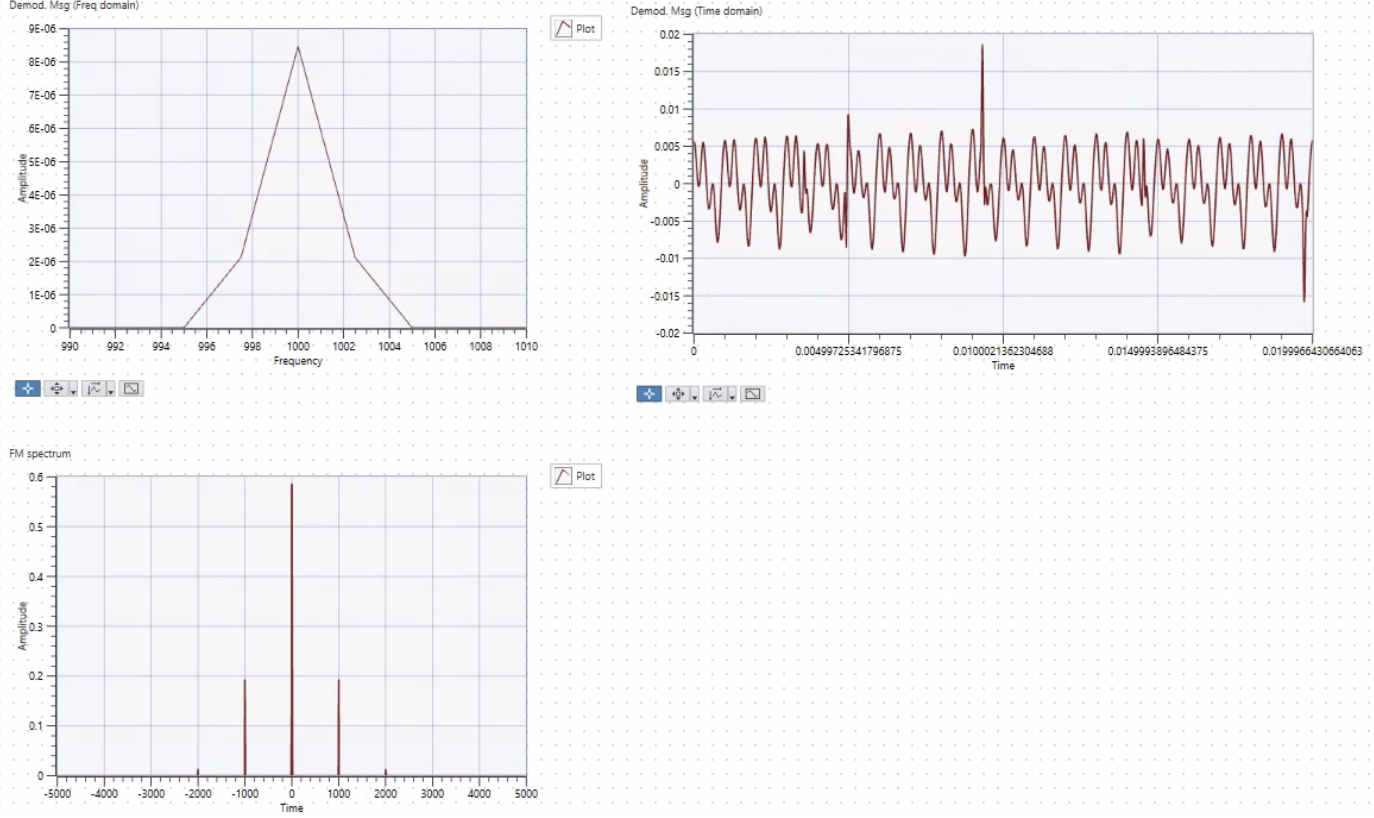
\includegraphics[width=0.7\textwidth]{deltaf_1k.png} \end{center}

\textbf{Observations ($\Delta_f = 1$\,kHz, $\beta = 1$):}
\begin{itemize}[leftmargin=1.5em]
  \item Spectrum is compact: a strong carrier peak at 0\,Hz with sidebands at $\pm 1$\,kHz.
  \item Measured bandwidth $\approx 4$\,kHz, matching Carson's prediction $B_T = 2(1+1) = 4$\,kHz.
  \item Very close to an AM spectrum (narrowband FM).
  \item The demodulated signal looks distorted (Poor SNR performance for low values of Deviation ratio, we know that SNR quadraticaly increases with the deviation ratio as seen in previous derivations).
\end{itemize}

\vspace{1em}

 \begin{center} 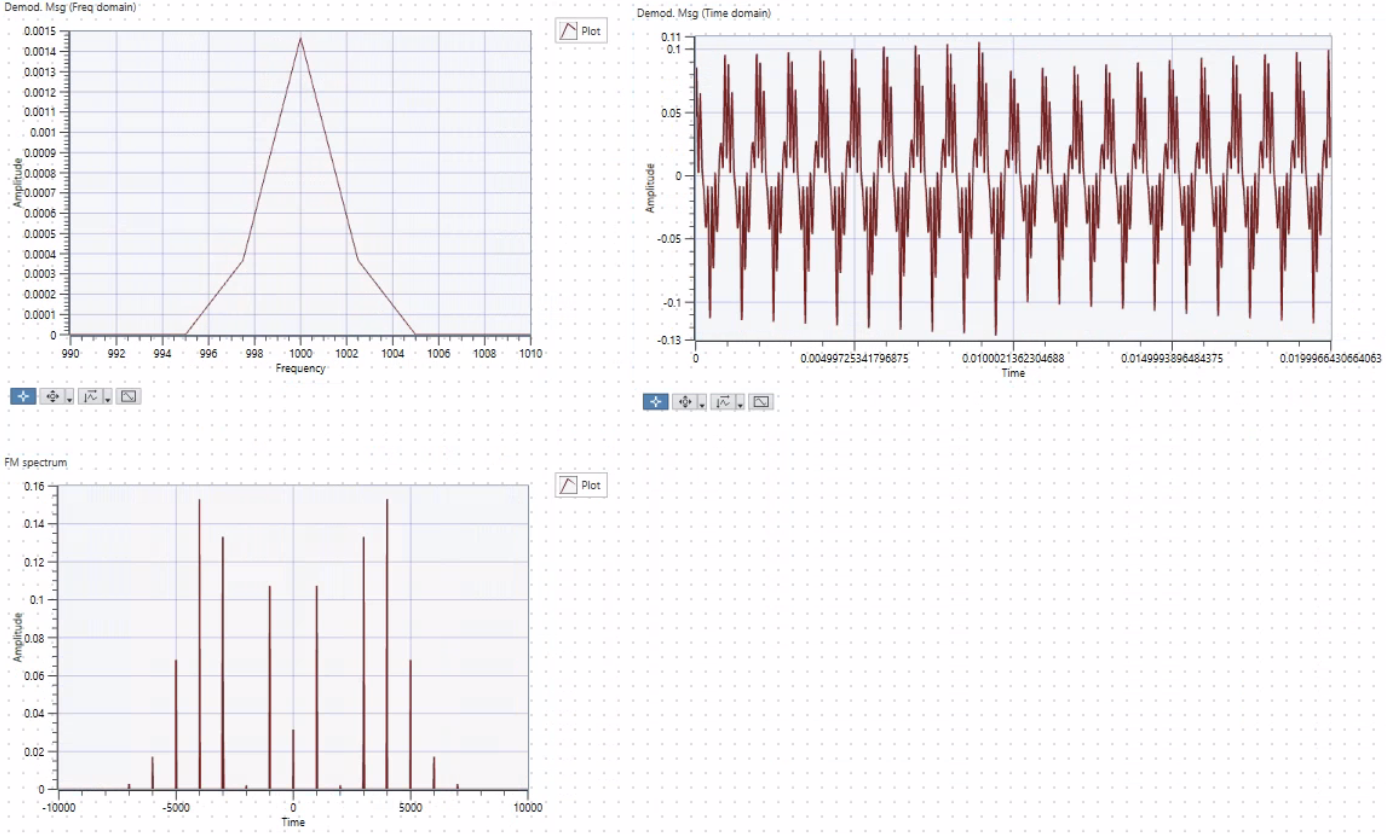
\includegraphics[width=0.7\textwidth]{deltaf_5k.png} \end{center}

\textbf{Observations ($\Delta_f = 5$\,kHz, $\beta = 5$):}
\begin{itemize}[leftmargin=1.5em]
  \item Multiple sidebands visible at $\pm 1, \pm 2, \ldots, \pm 6$\,kHz from the carrier.
  \item Measured bandwidth $\approx 14$\,kHz. Carson predicts $B_T = 2(5+1) = 12$\,kHz , measured is slightly wider due to outer Bessel sidebands.
  \item Clear wideband FM: energy is spread across many spectral lines.
    \item Better SNR performance but the signal is still distorted
\end{itemize}

\vspace{1em}

\begin{figure}[h]
\centering
\begin{minipage}{0.48\textwidth}
    \centering
    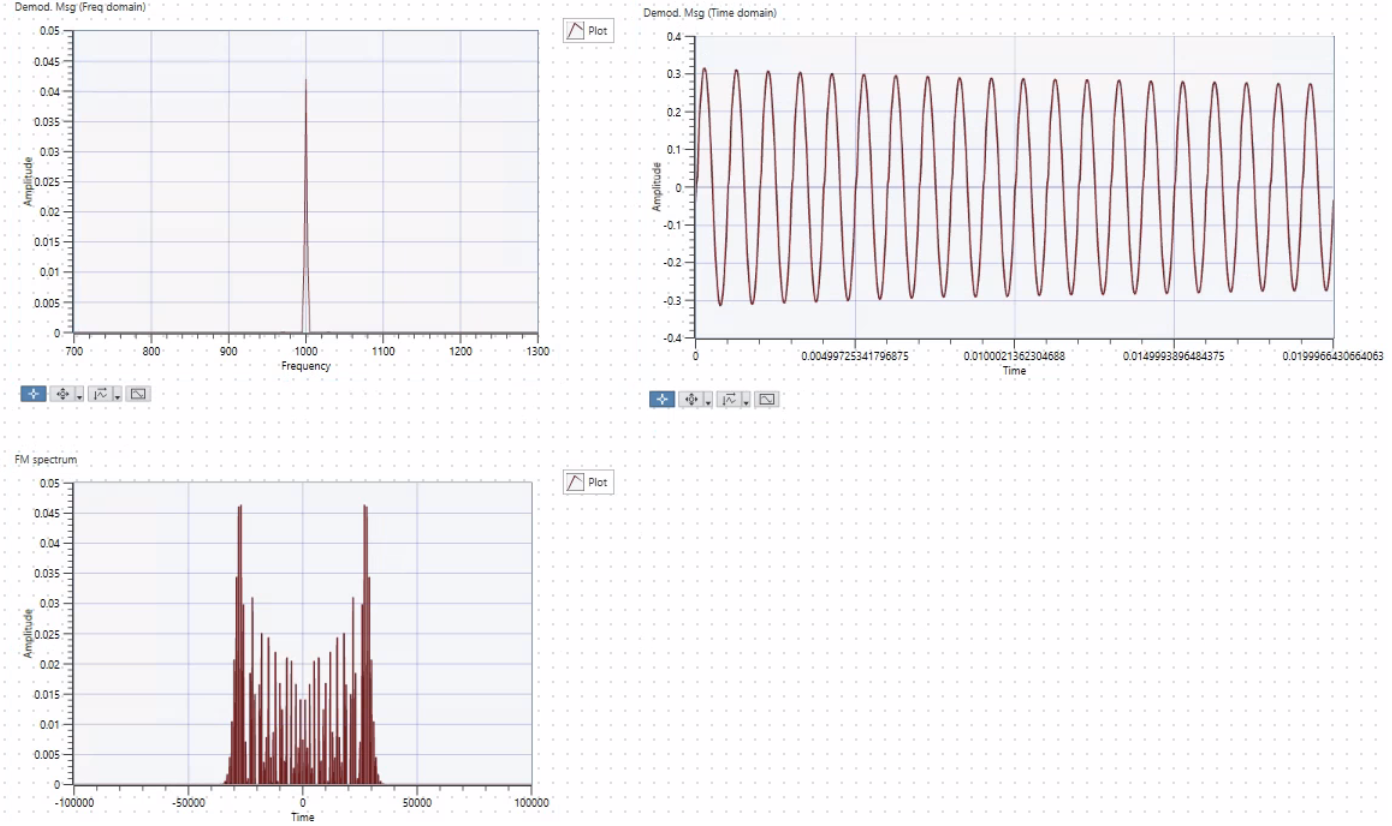
\includegraphics[width=\linewidth]{deltaf30k.png}
    \caption{First graph}
\end{minipage}
\hfill
\begin{minipage}{0.48\textwidth}
    \centering
    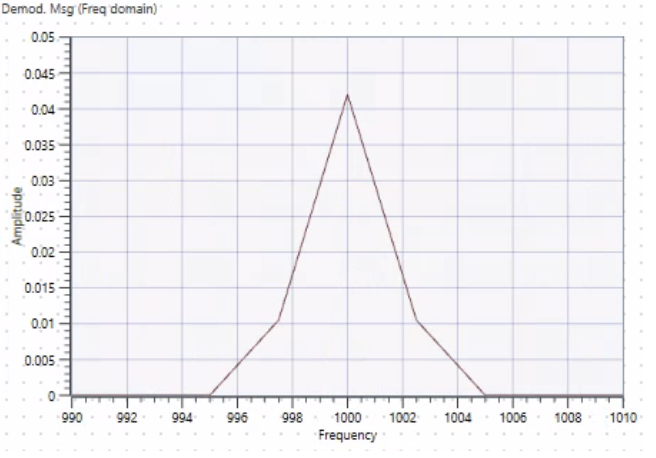
\includegraphics[width=\linewidth]{deltaf_30k(2).png}
    \caption{Second graph}
\end{minipage}
\end{figure}

\textbf{Observations ($\Delta_f = 30$\,kHz, $\beta = 30$):}
\begin{itemize}[leftmargin=1.5em]
  \item Very wide spectrum with many densely packed sidebands.
  \item Measured bandwidth $\approx 70$\,kHz. Carson predicts $B_T = 2(30+1) = 62$\,kHz, again, measured is wider.
  \item Very good SNR performance at the cost of Bandwith.
\end{itemize}

\begin{SummaryBox}[Exercise 4a Summary]
\begin{itemize}[leftmargin=1.5em]
  \item Carson's rule $B_T = 2(\Delta_f + W)$ gives a good \textbf{lower bound} on FM bandwidth.
  \item Measured bandwidths are wider due to outer Bessel sidebands not captured by the 98\% rule.
  \item As $\beta$ increases: more sidebands, wider spectrum, but higher output SNR ($\propto \beta^2$), the fundamental \textbf{bandwidth--SNR trade-off} of FM.
  \item Low $\Delta_f$ (low $\beta$) leads to narrowband FM with potential distortion at the demodulator.
\end{itemize}
\end{SummaryBox}

\newpage

\section{Exercise 5: Listening to FM Radio (Bonus): Conceptual Analysis}

\begin{GoalBox}[Goal of Exercise 5]
Use the USRP as an FM radio receiver: scan the commercial FM band (87.5--108\,MHz) to detect local stations, then tune in and listen to the demodulated audio.
\end{GoalBox}

\vspace{1em}

\subsection{5.1 \; Commercial FM Radio Context}

Commercial FM radio in the UK operates in the \textbf{VHF Band II (Very High Frequency)} (87.5--108\,MHz). Each station occupies a channel with $\Delta_f = 75$\,kHz and $W = 15$\,kHz (audio bandwidth), giving:
\[
  B_T = 2(75 + 15) = 180\,\text{kHz} \approx 200\,\text{kHz channel spacing}
\]

This corresponds to $\beta = 75/15 = 5$, which gives FM an SNR advantage of $3 \times 5^2 \times \frac{3}{2} = 15.7$\,dB over baseband.

\vspace{0.5em}

\subsection{5.3 \; AM vs.\ FM Performance Comparison}

\begin{KeyBox}[Key: Analog Modulation Comparison ]
\begin{center}
\renewcommand{\arraystretch}{1.3}
\begin{tabular}{lccc}
\toprule
\textbf{Scheme} & \textbf{SNR vs.\ baseband} & \textbf{Bandwidth $B_T$} \\
\midrule
Full AM    & $-4.8$\,dB worse  & $2W$ \\
DSB-SC     & Identical          & $2W$ \\
SSB        & Identical          & $W$ \\
FM ($\beta = 5$) & $+15.7$\,dB better & $2(\beta+1)W = 12W$ \\
FM + de-emphasis & $+28.7$\,dB better & $12W$ \\
\bottomrule
\end{tabular}
\end{center}
FM achieves much higher SNR by trading bandwidth. Pre-/de-emphasis adds another $\sim$13\,dB.
\end{KeyBox}

\newpage

\section{Exercise 5: Listening to FM Radio (Bonus): Task Answers}

\subsection{Task 1: Detecting FM Stations}

 \begin{center} 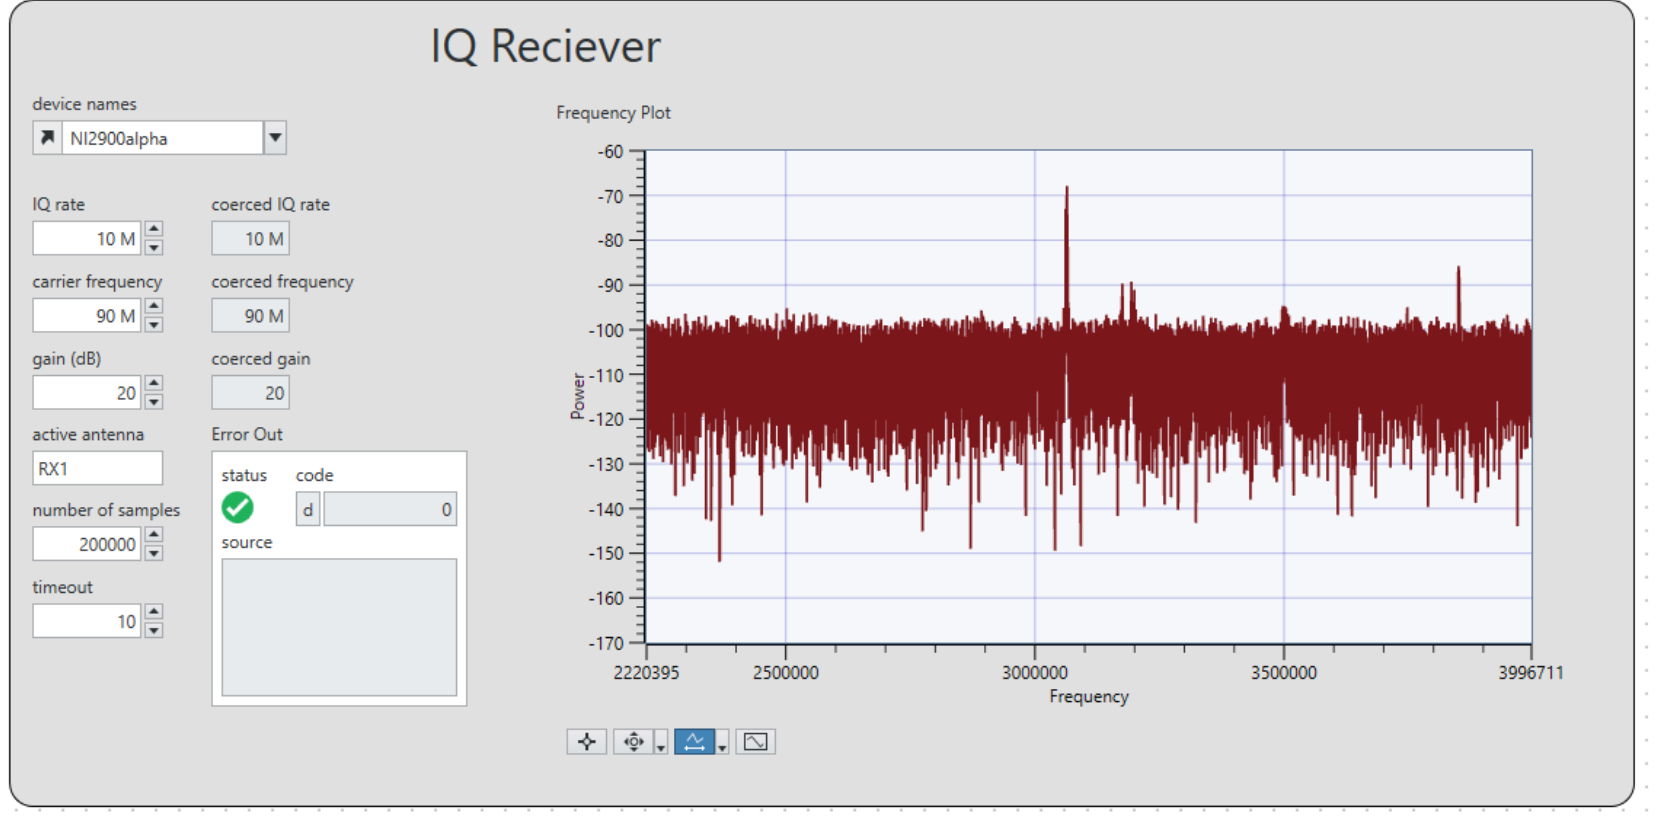
\includegraphics[width=0.7\textwidth]{bonusex5_1.png} \end{center}

  \begin{center} 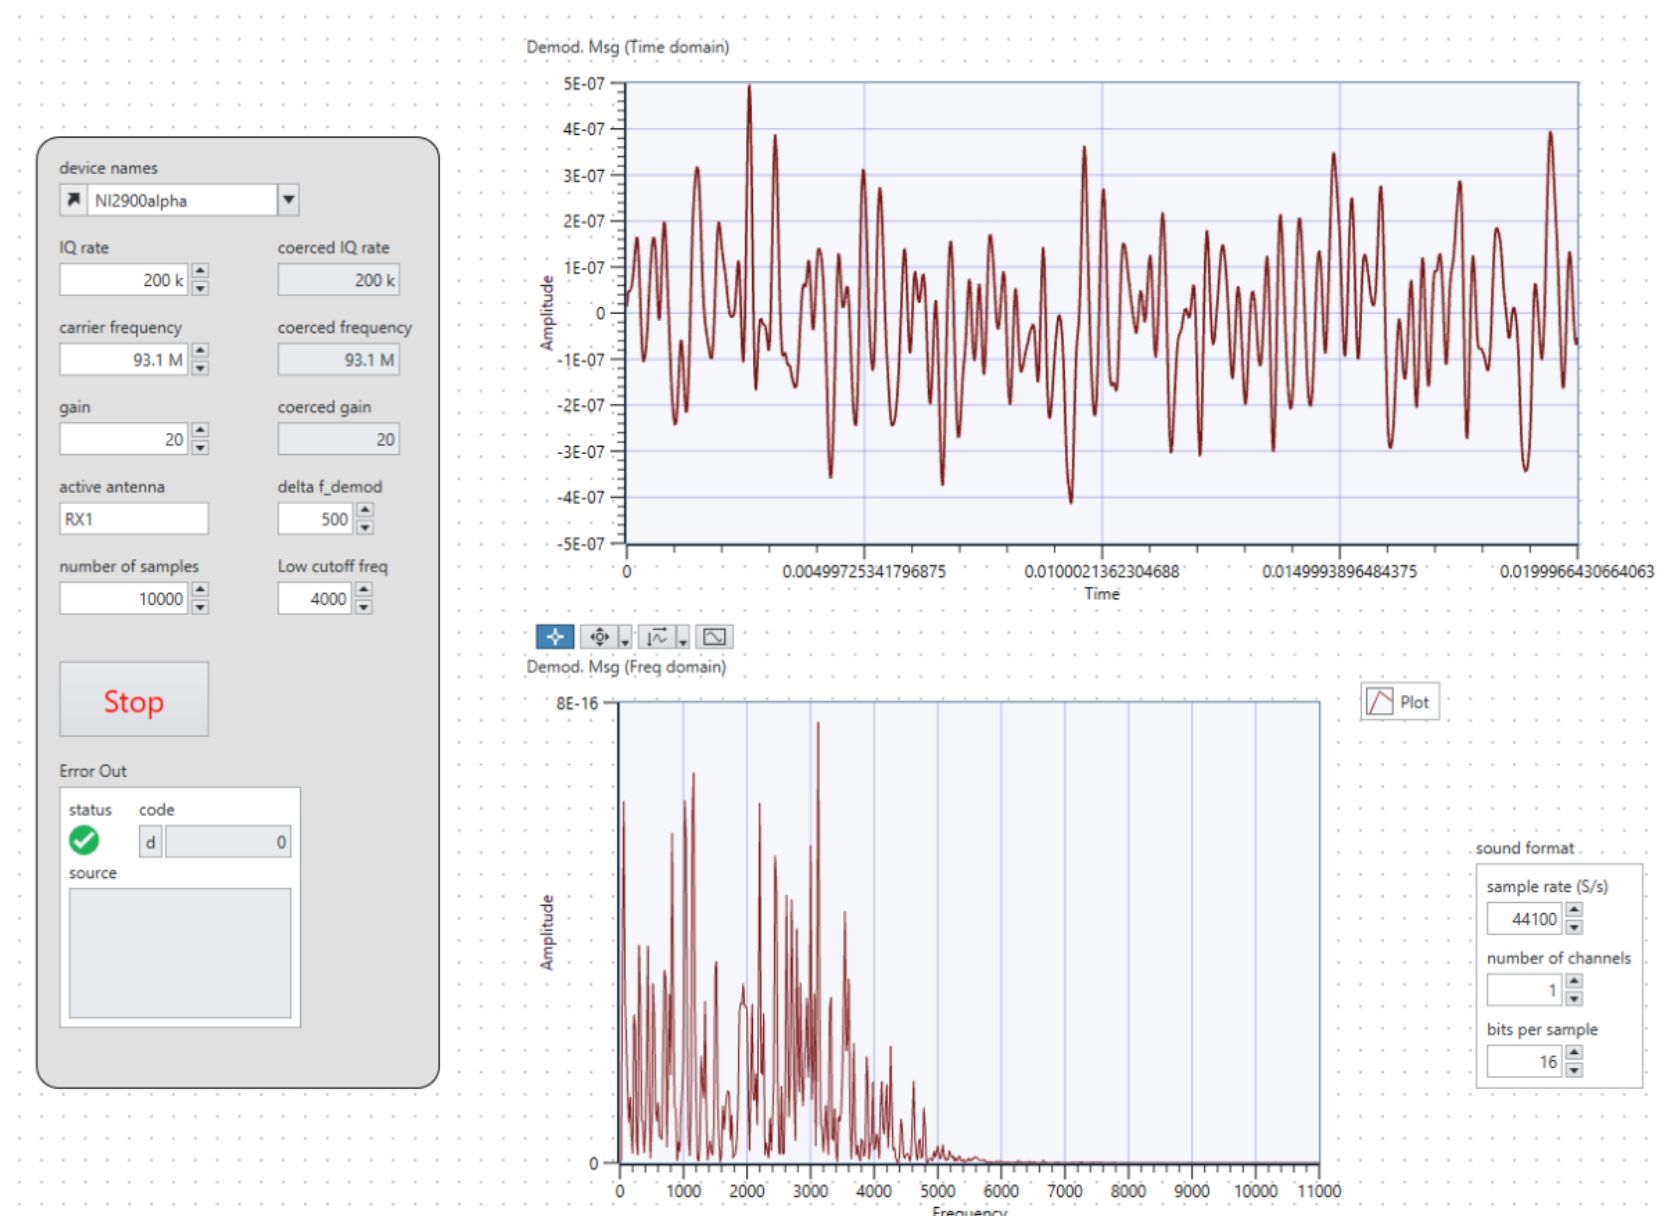
\includegraphics[width=0.7\textwidth]{bonusex5_2.png} \end{center}
\vspace{2cm}

\textbf{Observations:}
\begin{itemize}[leftmargin=1.5em]
  \item Multiple peaks visible in the power spectrum, each corresponding to an FM radio station.
  \item The strongest peak was at approximately $f = 93.1$\,MHz (the exact station varies by lab session, we tried this experiment multiple times).
  \item Increasing receiver gain reveals weaker stations, but also raises the noise floor.
\end{itemize}

\vspace{1em}

\subsection{Task 2: Listening to FM Audio}

\begin{itemize}[leftmargin=1.5em]
  \item Selected the strongest station frequency and entered it into \texttt{FM Music.gvi}.
  \item The demodulated audio was clearly audible through the speakers.
  \item Audio quality was good, consistent with the high SNR advantage of commercial FM ($\beta = 5 \Rightarrow$ 15.7\,dB above baseband).
\end{itemize}

\begin{SummaryBox}[Exercise 5 Summary]
\begin{itemize}[leftmargin=1.5em]
  \item The USRP can receive real commercial FM radio by tuning to the VHF band (87.5--108\,MHz).
  \item FM stations appear as peaks in the power spectrum; the strongest peak gives the best reception.
  \item Commercial FM uses $\beta = 5$ ($\Delta_f = 75$\,kHz, $W = 15$\,kHz), giving $B_T \approx 200$\,kHz per channel.
  \item FM's bandwidth--SNR trade-off is what makes it the standard for high-fidelity radio broadcast.
\end{itemize}
\end{SummaryBox}

\setcounter{secnumdepth}{2}

\end{document}
